\documentclass[
    12pt, 
    openright, 
    twside, 
    a4paper, 
    english, 
    brazil
]{abntex2}

% \usepackage{helvet}
% \renewcommand{\familydefault}{\sfdefault}

\usepackage[T1]{fontenc}	
\usepackage[utf8]{inputenc}		  %Caractes especiais
\usepackage{lastpage}			 	 % Usado pela Ficha catalográfica
\usepackage{indentfirst}			 % Indenta o 1º parágrafo de cada seção.
\usepackage{color}					  % Controle das cores
\usepackage{graphicx}				% Inclusão de gráficos
\usepackage{microtype}
% \usepackage{natbib}
% \usepackage{graphicx}
\usepackage{amsmath}
\usepackage{amssymb,amsfonts,amsthm}
\usepackage{setspace}
\usepackage{lipsum}				% para geração de dummy text
% ---
\usepackage[normalem]{ulem}
\usepackage{todonotes}
\usepackage{dirtytalk}
\usepackage[brazilian,hyperpageref]{backref}	 % Paginas com as citações na bibl
\usepackage[alf]{abntex2cite}	% Citações padrão ABNT

\renewcommand{\bf}[1]{\mathbf{#1}}
\renewcommand{\rm}[1]{\mathrm{#1}}
\usepackage{multirow}
\usepackage{cite}
\renewcommand\citeleft{[}
\renewcommand\citeright{]}
\usepackage{minted}
\renewcommand{\imprimircapa}{
\vfill
 \begin{center}
    

    {\large\bfseries UNIVERSIDADE FEDERAL DA BAHIA} \\
    
   
    {\large\bfseries CAMPUS ONDINA}  \\ 

    \vspace*{1in}
    \begin{large} \bfseries João Pedro Rodrigues Cerqueira \end{large}\\[0.4in]

    \vspace*{4cm}
    \noindent \\
    
    \large\bfseries{MeForma: uma aplicação web para acompanhamento da evolução acadêmica de estudantes de graduação} \\
    \vfill
    \large\bfseries{ SALVADOR \\ 2018}
\end{center}

\normalsize
}
\renewcommand{\imprimirfolhaderosto}{

\begin{center}

    {\large JOÃO PEDRO RODRIGUES CERQUEIRA\\}
    \vspace{8cm}
    {\Large \textsc\textbf{{MeForma: uma aplicação web para acompanhamento da evolução acadêmica de estudantes de graduação} }\\}
    \vspace{1cm}
    \hspace{.45\linewidth}
    \begin{minipage}{.50\linewidth}

            \textbf{Trabalho de Conclusão de Curso submetido à Universidade Federal da Bahia,  como requisito 
            necessário para obtenção do grau de Bacharel em Ciência da Computação }

           
    
    \end{minipage}

    \vspace{2cm}
    \vfill
    {\large Salvador, 2018}
\end{center}

}
% ---
% Configurações do pacote backref
% Usado sem a opção hyperpageref de backref
\renewcommand{\backrefpagesname}{Citado na(s) página(s):~}
% Texto padrão antes do número das páginas
\renewcommand{\backref}{}
% Define os textos da citação
\renewcommand*{\backrefalt}[4]{
	\ifcase #1 %
		Nenhuma citação no texto.%
	\or
		Citado na página #2.%
	\else
		Citado #1 vezes nas páginas #2.%
	\fi}%
	
\definecolor{blue}{RGB}{41,5,195}
\makeatletter
\hypersetup{
     	%pagebackref=true,
		colorlinks=true,       		% false: boxed links; true: colored links
    	linkcolor=blue,          	% color of internal links
    	citecolor=black,        		% color of links to bibliography
    	filecolor=magenta,      		% color of file links
		urlcolor=blue,
		bookmarksdepth=4
}

\makeatother
% --- 
% Espaçamentos entre linhas e parágrafos 
% --- 

% O tamanho do parágrafo é dado por:
\setlength{\parindent}{1.3cm}

% Controle do espaçamento entre um parágrafo e outro:
\setlength{\parskip}{0.2cm}  % tente também \onelineskip

\makeindex

\usepackage{float}
\begin{document}
\selectlanguage{brazil}
\frenchspacing 
\pretextual
\imprimircapa
\imprimirfolhaderosto
\begin{folhadeaprovacao}


\begin{center}


            {UNIVERSIDADE FEDERAL DA BAHIA} \\
           

    \vspace{1.5cm}
                                    {JOÃO PEDRO RODRIGUES CERQUEIRA}\\
    \bfseries{}
\end{center}

Esta Monografia foi julgada adequada para a obten\c{c}\~{a}o do título  de Bacharel em Ciência da Computação, sendo aprovada em sua forma final  pela banca examinadora:

    \vspace{3cm}
    \assinatura{Orientador \\ Prof. Dr. Tiago de Oliveira Januario \\ Universidade Federal da Bahia - UFBA}
    \assinatura{Prof. Dr. Ivan do Carmo Machado \\ Universidade Federal da Bahia - UFBA}
    \assinatura{Prof. Dr. Rodrigo Rocha Gomes e Souza \\ Universidade Federal da Bahia - UFBA}
    
    \vspace{3 cm}%\vfill

    \begin{center}
        Salvador, \today
    \end{center}
  
\end{folhadeaprovacao}
% ---
% Agradecimentos
% ---
\begin{agradecimentos}
Agradeço primeiramente a Deus por me conceder vida, saúde, sabedoria e paciência para cursar uma graduação no Brasil, em especial na Universidade Federal da Bahia. Em segundo lugar, aos meus pais que me deram suporte até onde suas mãos puderam alcançar para que eu não desistisse dessa jornada, em especial à minha mãe que me alfabetizou e educou com todas as dificuldades enquanto mulher negra e mãe solteira, e me deu espaço para que eu pudesse explorar minha criatividade e sonhar. Ademais à InfoJr UFBA que me acolheu enquanto estudante sem muita noção do que esperar do curso, me deu uma profissão que me permitiu continuar estudando, me apresentou novas visões de mundo e acima do profissional me educou para uma vida adulta mais consciente sobre mim e sobre os outros, e me presenteou com parceiros e histórias inesquecíveis. Por fim, ao meu orientador Tiago Januário por acreditar no meu trabalho e apoiar a realização do mesmo.

\end{agradecimentos}
% ---
% ---
% RESUMOS
% ---

% resumo em português
\setlength{\absparsep}{18pt} % ajusta o espaçamento dos parágrafos do resumo
\begin{resumo}
É difícil para o estudante ter ciência de sua evolução no curso de graduação sem o auxílio de uma ferramenta adequada. Pensando nisso, foi desenvolvido um sistema chamado MeForma. O MeForma tem o objetivo de apoiar e facilitar a vida acadêmica dos estudantes de graduação da Universidade Federal da Bahia, tornando-os mais participativos de sua própria formação, esclarecendo os passos necessários para atingí-la e ajudando-os a se orientar com relação a esses passos. Este trabalho traz uma reformulação completa do MeForma, com novas funcionalidades e correções de problemas como a limitação com relação ao alcance de usuários, problemas de usablidade e portabilidade, além de trazer uma avaliação sobre a qualidade da nova versão. A nova versão foi desenvolvida com preocupações modernas e recursos voltados a atender o maior número de estudantes de graduação possível.

 \textbf{Palavras-chave}: Universidade Federal da Bahia, formatura, extração de dados da web, aplicação híbrida, desempenho acadêmico.
\end{resumo}

% resumo em inglês
\begin{resumo}[Abstract]
 \begin{otherlanguage*}{english}
It is difficult for an student to be aware of his evolution in the undergraduate course without the aid of a suitable tool. Thinking about it, a system called MeForma was developed. MeForma aims to support and facilitate the academic life of undergraduate students at Federal University of Bahia, making them more participatory in their own training, clarifying the steps necessary to reach it and helping them to orient themselves in relation to those steps. This work brings a complete redesign of the MeForma, with new functionalities and fixes of problems such as limitation regarding user reach, usability and portability problems, as well as an evaluation of the quality of the new version. The new version was developed with modern concerns and resources aimed at serving as many undergraduate students as possible.

   \vspace{\onelineskip}
   \noindent 
   \textbf{Keywords}: Federal University of Bahia, graduation, web data extraction, hybrid apps, academic performance.
 \end{otherlanguage*}
\end{resumo}

%% resumo em francês 
%\begin{resumo}[Résumé]
% \begin{otherlanguage*}{french}
%    Il s'agit d'un résumé en français.
% 
%   \textbf{Mots-clés}: latex. abntex. publication de textes.
% \end{otherlanguage*}
%\end{resumo}
%
%% resumo em espanhol
%\begin{resumo}[Resumen]
% \begin{otherlanguage*}{spanish}
%   Este es el resumen en español.
%  
%   \textbf{Palabras clave}: latex. abntex. publicación de textos.
% \end{otherlanguage*}
%\end{resumo}
% ---
% ---
% Lista de ilustrações
% ---
\pdfbookmark[0]{\listfigurename}{lof}
\listoffigures*
\cleardoublepage
%% ---
% Lista de Tabelas
\pdfbookmark[0]{\listtablename}{lot}
\listoftables*
\cleardoublepage
% ---
\include{siglas}
% ---
% inserir o sumario
%% ---
\pdfbookmark[0]{\contentsname}{toc}
\tableofcontents*
\cleardoublepage
%% ---



% ----------------------------------------------------------
% ELEMENTOS TEXTUAIS
% ----------------------------------------------------------
\textual

\chapter{Introdução}

As aplicações Web acompanham a vida acadêmica dos estudantes da Universidade Federal da Bahia. Diversas aplicações trazem um conjunto de informações que são relevantes para a trajetória do estudante dentro da universidade, como por exemplo, disciplinas ofertadas por semestre, calendário acadêmico, regimentos e grade curricular. Contudo, a universidade não provê nenhum sistema que se preocupe em transparecer para o discente o quão próximo ele está da formatura, ou o que é necessário para alcançá-la. Nesse cenário, surge o MeForma.

A ideia do MeForma é tornar o estudante mais participativo e preocupado com a sua formação, permitindo que ele possa acompanhar seu desempenho no curso a partir de seus dados acadêmicos, como disciplinas cursadas e cargas horárias aproveitadas. Esses dados são inseridos pelos próprios usuários, computados pelo sistema e exibidos em forma de porcentagem de completude do curso.

O ponto de partida do MeForma foi uma planilha, criada em 2015, que servia de apoio a dois estudantes do curso de Ciência da Computação da UFBA. Através da planilha, é possível acompanhar a porcentagem de disciplinas obrigatórias concluídas, a porcentagem de carga horária optativa, e a porcentagem de carga horária complementar. Em 2016, foi lançado um aplicativo para o sistema Android com a intenção de compartilhar os benefícios trazidos pela utilização da planilha com todos os estudantes da UFBA. E, em 2018, surgiu o desafio de reconstruir o MeForma com base nas necessidades e melhorias apontadas pelos usuários durante o tempo de vida do aplicativo já lançado. O novo sistema é chamado neste trabalho de MeForma2 e está disponível para as plataformas Web e Android.

O MeForma2, no que diz respeito ao software, veio com o objetivo de melhorar a portabilidade e a usabilidade da aplicação, permitindo que mais pessoas pudessem utilizá-la em seus dispositivos e que essa utilização fosse fácil e agradável. Para resolver as questões de portabilidade, foi desenvolvida uma versão Web do MeForma2, levando em consideração o fato de que aplicações Web podem ser executadas em qualquer dispositivo capaz de executar um navegador da Web. Para resolver as questões de usabilidade, um novo leiaute foi pensado com base em outras aplicações e nas opiniões dos usuários da primeira versão  do MeForma.

Dentre os desafios da versão Web estavam a responsividade da aplicação e a compatibilidade dos recursos em JavaScript, maior parte do aplicativo, com os navegadores disponíveis. Essas e outras questões foram resolvidas com o uso do Ionic Framework, um \textit{framework} para desenvolvimento de aplicativos híbridos responsivos. O Ionic é responsável por garantir a compatibilidade do código em JavaScript com as versões mais recentes dos navegadores mais populares do mundo. Além disso, o Ionic oferece recursos para que o aplicativo seja responsivo, ou seja seja compatível com qualquer tamanho de tela.

Pra mensurar a qualidade da aplicação, foram coletados dados utilizando as seguintes ferramentas: uma avaliação heurística, para avaliar a usabilidade da interface; uma avaliação de relevância da aplicação, para entender se a aplicação é útil em seu propósito; uma pesquisa de satisfação dos usuários, para avaliar o quão confortáveis os usuários estão com a utilização da aplicação; sugestões enviadas por usuários, para que a aplicação pudesse crescer com base na experiência de quem a utiliza; e estatísticas de uso da aplicação, para entender o comportamento dos usuários.

Como auxiliar na construção do MeForma2, foi construído um Web Scraping apelidado de CMF para explorar os dados de cursos, currículos e disciplinas da UFBA vistos como necessários para a aplicação. Graças ao CMF, o MeForma2 contemplou os 100 cursos de graduação da UFBA (sendo 93 cursos de Salvador e 7 de Vitória da Conquista), contra 79 da primeira versão; 112 currículos de cursos, contra 79 da primeira versão do MeForma; e 5419 disciplinas, contra 4966 da primeira versão.

O MeForma2 inclui um painel de monitoramento dos cursos apelidado de MFPAC, o qual utiliza os dados coletados pelo MeForma2 para oferecer à liderança dos cursos informações sobre o desempenho dos estudantes que possam embasar e auxiliar nas tomadas de decisão e execuções de ações administrativas a respeito dos cursos, além de contribuir com processos de orientação acadêmica individual.

O desenvolvimento do MeForma2 foi iniciado no dia 12 de Julho de 2018, e a aplicação foi liberada para o público no dia 28 de Outubro de 2018, Totalizando 109 dias de desenvolvimento, incluindo o dia inicial. Os dados coletados dos usuários do MeForma2 foram coletados entre os dias 28 de Outubro de 2018 e 16 de Novembro de 2018.

\chapter{Justificativa}

O MeForma2 é um sistema cuja principal motivação é apoiar a vida acadêmica dos estudantes de graduação da UFBA, ajudando-os a se orientar com relação à conclusão de seus respectivos cursos, partindo da hipótese de que é difícil para o estudante ter ciência de sua evolução no curso de graduação sem o auxílio de uma ferramenta adequada. 

Nesse cenário, enquanto ferramenta de orientação, o MeForma2 serve para facilitar a passagem de um estudante pelo curso de graduação, deixando ele alerta sobre o que é necessário para concluir o currículo do curso e o quanto ele está progredindo semestre a semestre.

Com a inclusão do MFPAC, o MeForma2 se torna uma ferramenta muito útil para os colegiados e departamentos responsáveis por cada curso, pois através dos dados inseridos no MeForma2 pelos estudantes, é possível obter uma série de informações sobre o desempenho dos mesmos e visualizá-las no MFPAC. Essas informações podem contribuir para a execução de ações administrativas, por parte da liderança acadêmica, que melhorem os cursos, o desempenho dos estudantes e, por consequência, a avaliação dos cursos.

Os cursos de graduação no Brasil são avaliados pelo SINAES -- Sistema Nacional de Avaliação de Educação Superior. O SINAES Foi criado pela Lei n° 10.861, de 14 de abril de 2004, e é formado por três componentes principais: a avaliação das instituições, dos cursos e do desempenho dos estudantes. Os resultados da avaliação possibilitam traçar um panorama da qualidade dos cursos e instituições de educação superior no país.

Nesse cenário, o MeForma2 é uma ferramenta capaz de contribuir para que os cursos de graduação da UFBA melhorem sua avaliação perante os órgãos avaliadores a partir de insumos reais específicos sobre o desempenho dos estudantes em cada disciplina, podendo influenciar em adequações de grade curricular, oferta de disciplinas, escalonamento de professores, dentre outros aspectos aos quais os números gerados pelo sistema dizem respeito.
\chapter{Aplicação}
\section{Passos Iniciais}
O controle da evolução acadêmica torna-se uma tarefa difícil de ser executada quando o estudante não possui um sistema de controle acadêmico confiável. Nesse cenário, surge o MeForma. O MeForma é um sistema web que começou como uma planilha, no ano de 2015, que servia de apoio a dois estudantes do curso de Ciência da Computação da UFBA para registro de disciplinas concluídas e controle de carga horária. A planilha continha todas as disciplinas existentes na grade do curso. Em 2016, iniciou-se o desenvolvimento de um aplicativo mobile para que os benefícios trazidos pela utilização da planilha pudessem ser compartilhados com todos os estudantes da UFBA. Com o lançamento da aplicação e a utilização dos estudantes, foram apontadas falhas e necessidades de melhoria através de feedbacks enviados por e-mail, pelo aplicativo ou de forma mais informal em conversas diretas com o desenvolvedor.
Os feedbacks se tornaram requisitos de desenvolvimento de software, e foram:
\begin{itemize}
\item Criação de uma versão WEB (acessível por navegador) - uma vez que a aplicação é acessada normalmente em início e fim de semestre letivo, não é bom manter o usuário preso a uma necessidade de instalação.
\item Inclusão de todos os cursos de graduação da UFBA.
\item Inclusão de diferentes currículos para um mesmo curso - O sistema considerava apenas o currículo vigente de cada curso, ignorando o fato de que um curso pode ter muitos currículos. Isso excluía os estudantes que não estavam matriculados no currículo vigente no momento de criação do curso da possibilidade de utilizar o sistema.
\item Informações sobre os pré-requisitos das disciplinas - o sistema deveria permitir que os usuários consultassem os pré-requisitos das disciplinas de um curso.
\item Permitir o registro do semestre corrente - Os usuários não querem saber apenas o quanto já atingiram com relação à completude de um curso, eles querem saber também o quanto podem atingir, caso sejam aprovados nas disciplinas que estão cursando.
\item Permitir recuperar dados do SIAC WEB - Os usuários julgaram mais confortável que a aplicação pudesse importar os dados já disponíveis no portal do aluno, o SIAC WEB.
\item Permitir que os responsáveis pelos cursos pudessem acompanhar o desempenho dos alunos de acordo com o MeForma.
\end{itemize}

Com base nos feedbacks e nos requisitos levantados, decidiu-se criar uma nova versão, mais completa e mais agradável para o MeForma, o MeForma2.

\section{Tecnologias Utilizadas}
\label{tecnologias}
Esta seção lista as tecnologias que foram utilizadas para a escrita de todo o código fonte do MeForma2. Após a definição dos requisitos para a criação do novo projeto, iniciou-se a etapa de escolha das tecnologias para escrita da nova versão. Optou-se por continuar com a combinação que já havia sido empregada na versão anterior do MeForma, a fim de tornar mais simples o processo de migração do antigo sistema e de aproveitar ao máximo o código que já existia. As tecnologias escolhidas foram as seguintes: Ionic Framework, PHP, MySQL, Apache2.

O Ionic Framework, ou apenas Ionic, é uma ferramenta para desenvolvimento de aplicativos que permite gerar instaláveis ou interpretáveis para diversas plataformas, utilizando-se de uma única base de código. Esse tipo de aplicativo é conhecido como aplicativo híbrido.

Os aplicativos híbridos são websites executados em um shell de navegador através de um empacotador que tem acesso à camada de plataforma nativa dos dispositivos. Aplicativos híbridos têm muitos benefícios em relação a aplicativos nativos puros, especificamente em termos de suporte de plataforma e velocidade de desenvolvimento.

A grande vantagem em se utilizar o Ionic é que o código fonte pode ser escrito em linguagens de desenvolvimento WEB, a saber, HTML5, CSS3 e JavaScript. O termo é ``pode ser escrito'', porque a ferramenta incorpora outras tecnologias comuns na comunidade de desenvolvimento WEB e que facilitam o uso das linguagens citadas. São elas:
\begin{itemize}
\item Angular 2: O Angular é um framework que tem como objetivo resolver os principais desafios do desenvolvimento web e, nessa aplicação, ele é utilizado para realizar atualização automática do conteúdo das páginas HTML sem necessidade de recarregamento.
\item SASS: O sass é um pré-processador de CSS, o que significa dizer que o código é escrito em um formato no SASS, depois a ferramenta processa esse código e transforma-o em CSS, para que o interpretador final seja capaz de reconhecê-lo. A principal característica do SASS é que ele permite a inclusão de lógica de programação nos arquivos de estilização, oferecendo recursos como operadores condicionais, laços de repetição, e elementos do paradigma de programação orientada a objetos.
\item TypeScript: O TypeScript é um pré-processador que lida com a linguagem JavaScript. A principal característica do TypeScript é que ele permite a aplicação do paradigma de orientação a objetos de uma forma mais amigável para a linguagem JavaScript. A justificativa para a utilização dessa ferramenta é que a orientação a objetos nativa do JavaScript é muito diferente da que é aplicada por outras linguagens de programação.
\end{itemize}
O Ionic foi escolhido para o desenvolvimento do MeForma2 por causa da facilidade de configuração do ambiente de desenvolvimento e simplicidade de escrita do código fonte.

O Cordova, no que compõe esta aplicação, funciona como um empacotador para o código produzido em Ionic. O cordova foi escolhido por recomendação da documentação do Ionic Framework. Toda a documentação do Ionic é escrita com base nos recursos desenvolvidos para o Cordova.

O PHP é uma linguagem de programação que se caracteriza como uma linguagem de script de uso geral especialmente adequada para desenvolvimento web. Essa foi a linguagem server-side escolhida, pois a primeira versão do MeForma foi escrita com ela, então assumiu-se que a transição seria mais flúida se a nova versão também fosse escrita com o PHP. Além disso, levou-se em consideração a popularidade do PHP que faz com que ele tenha uma comunidade forte e ativa, além de uma lista vasta de servidores compatíveis disponíveis.

O  MySQL é um sistema de gerenciamento de banco de dados (SGBD), que utiliza a linguagem SQL (Linguagem de Consulta Estruturada, do inglês \textit{Structured Query Language}) como interface.
O MySQL foi escolhido por causa da experiência prévia do desenvolvedor com a utilização da tecnologia. Foi levado em consideração também a compatibilidade do MySQL com os serviços de servidor disponíveis no mercado e a compatibilidade com a linguagem de programação escolhida, o PHP.

\section{Funcionamento}
A seguir será descrito o funcionamento do MeForma2, no que diz respeito às telas disponibilizadas aos estudantes. Cada uma das subseções desta seção mostrará passos fundamentais a serem executados por um usuário para que o acompanhamento de seu desempenho ocorra. 
% A saber:
% \begin{enumerate}
% \item Cadastro e escolha do curso;
% \item Seleção de disciplinas concluídas;
% \item Cadastro de carga horária extra;
% \item Registro de semestre.
% \end{enumerate}
\subsection{Cadastro e Escolha do Curso}
Ao acessar a página inicial da aplicação, os usuários se deparam com a tela de login, que tem a opção de criar uma nova conta. Ao selecionar a opção de criação de conta, o usuário é encaminhado para um formulário de cadastro, que solicita alguns dados e exige a seleção de 3 componentes fundamentais para a aplicação. São eles:
\begin{itemize}
\item A universidade em que o usuário estuda.
\item O curso que ele exerce na universidade.
\item O currículo referente ao curso.
\end{itemize}
Após o preenchimento do formulário, o usuário é encaminhado novamente para a tela que contém o formulário de login, onde ele precisa inserir as credenciais que cadastrou para poder avançar no sistema. A Figura \ref{login} exibe, da esquerda para a direita, as telas de login e cadastro.
\begin{figure}[H]
	   \centering
	   		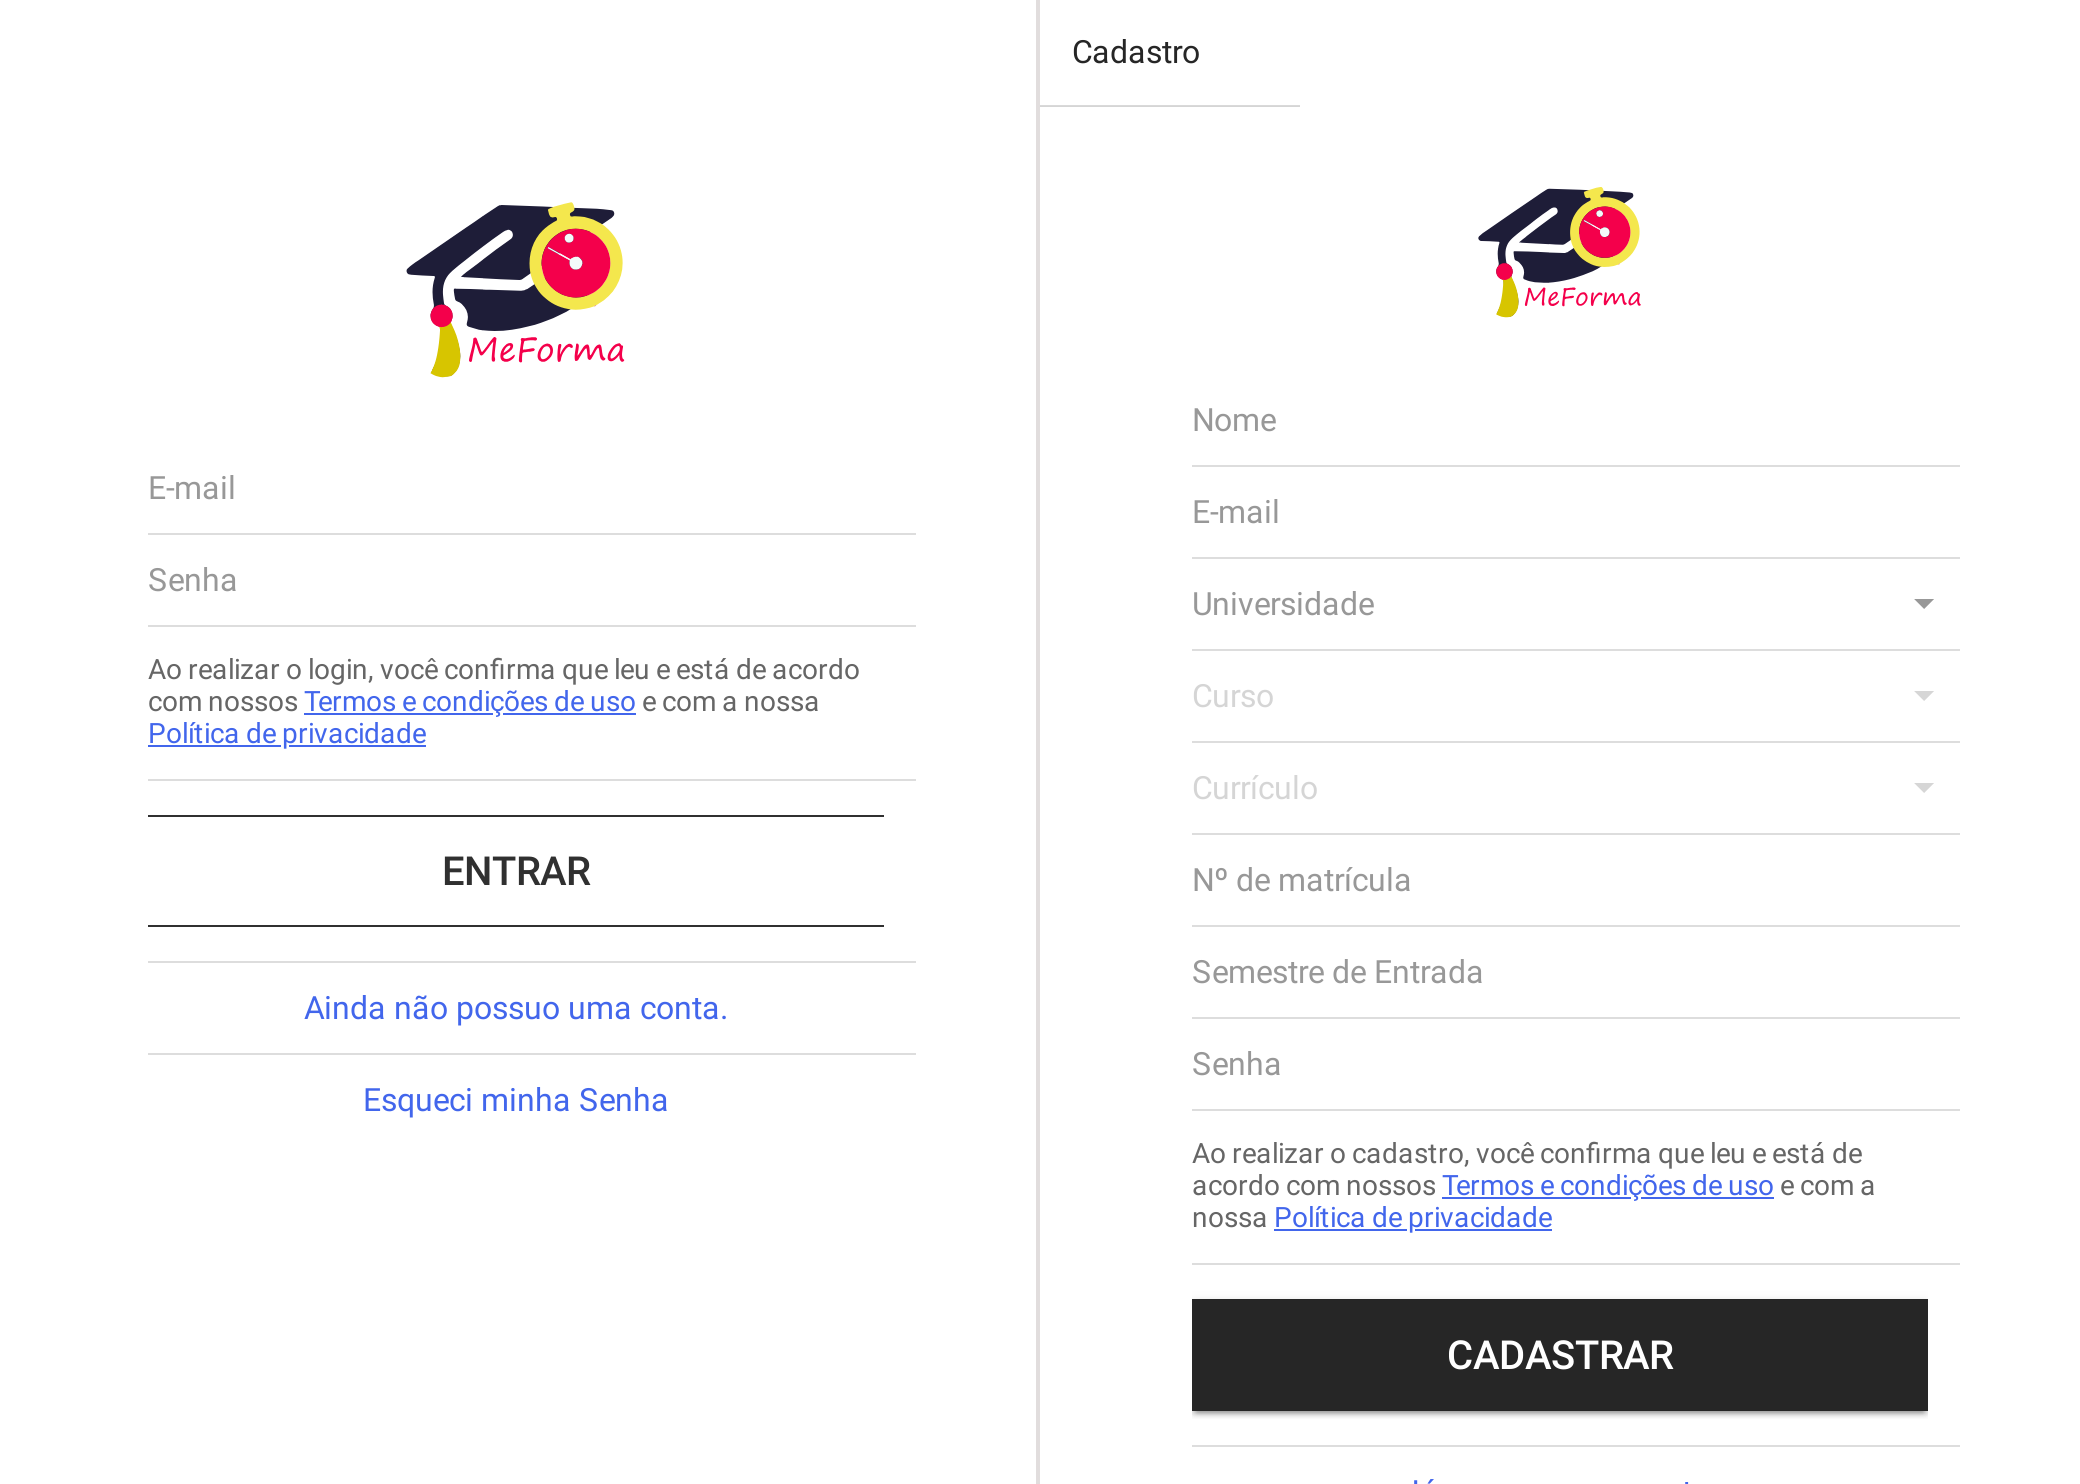
\includegraphics[scale=0.25]{pics/c3/1-login.png}
	   \caption{Tela de Login e Tela de Cadastro}
	   \label{login}
\end{figure}

\subsection{Visualização de Conclusão de Curso}
Após o login bem sucedido, o usuário é direcionado para a tela inicial do sistema, onde ele pode acompanhar a porcentagem de conclusão de cada elemento requisitado para conclusão do curso, além da porcentagem total de conclusão (Figura~\ref{completude}).
\begin{figure}[H]
	   \centering
	   		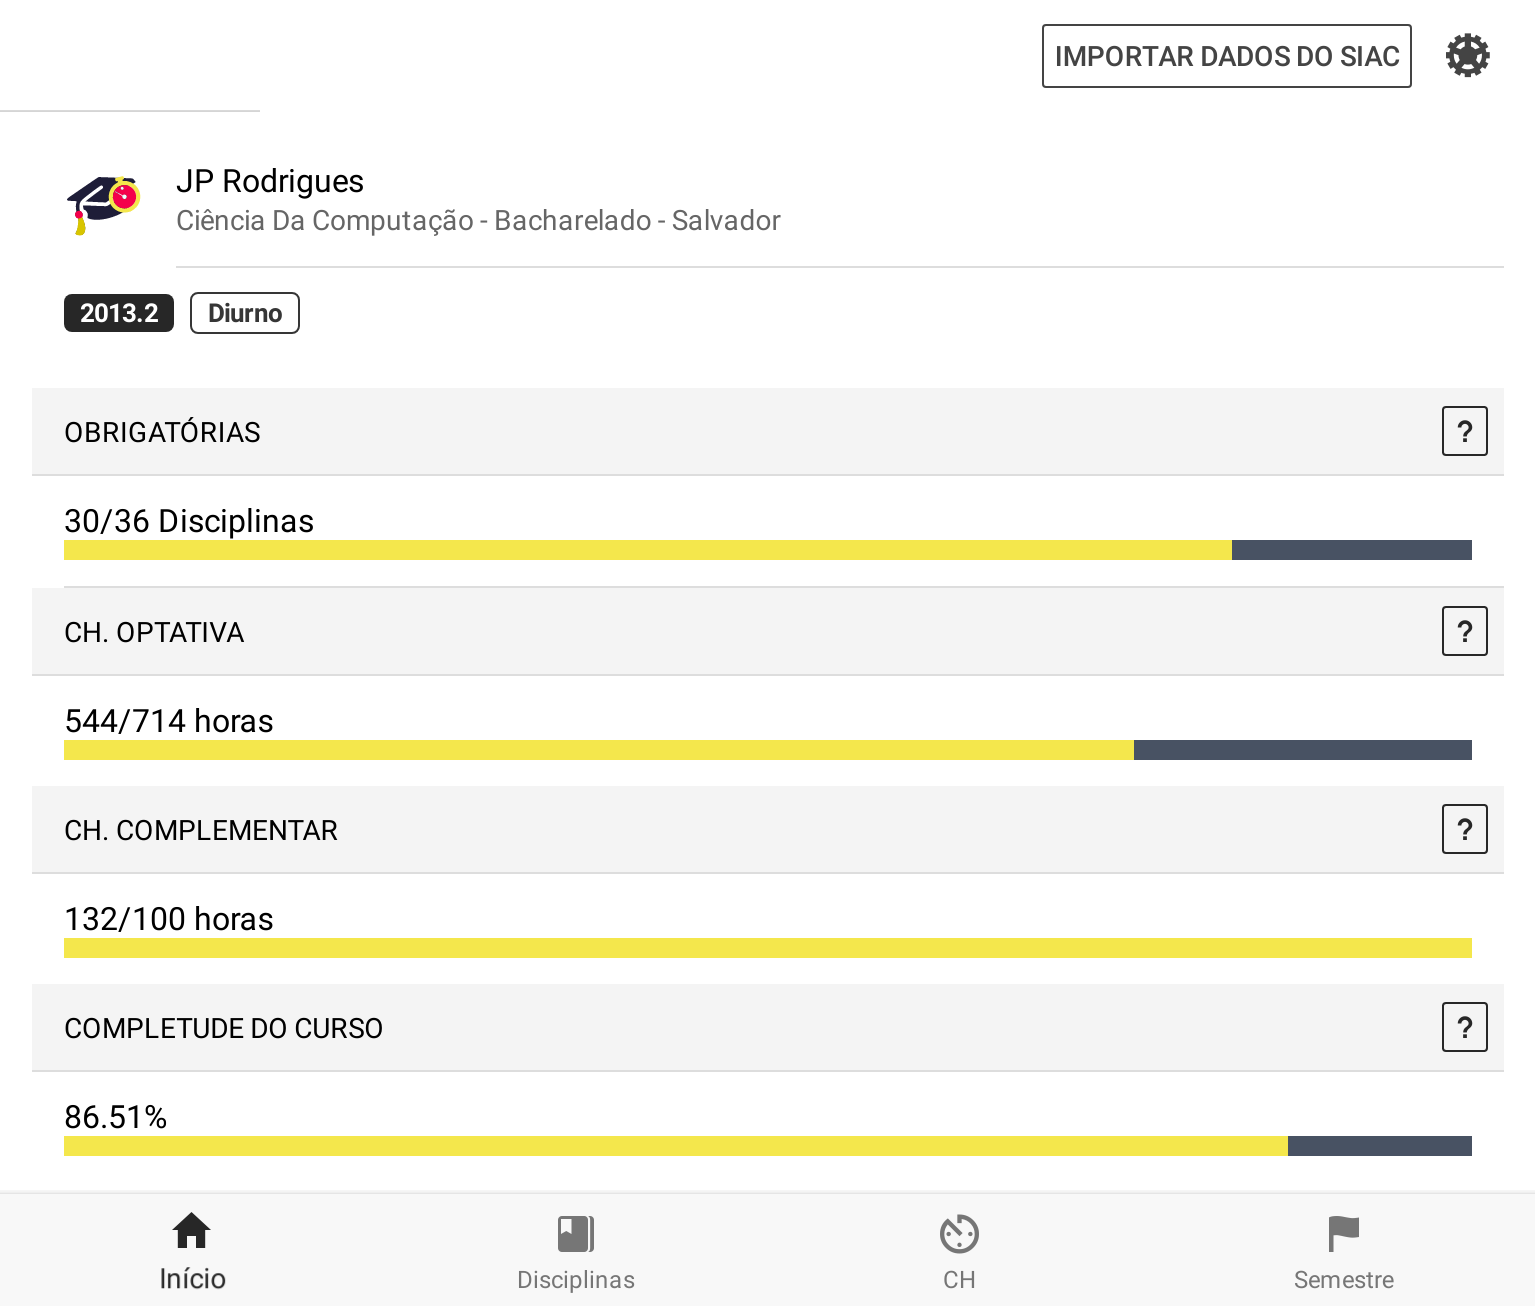
\includegraphics[scale=0.25]{pics/c3/3-completude.png}
	   \caption{Tela de completude do curso.}
	   \label{completude}
\end{figure}

\subsection{Seleção de Disciplinas Concluídas}
\label{disciplinas_tela}
Fundamental para o cumprimento do objetivo do sistema, essa é uma tela acessada ao clicar-se em ‘Disciplinas’, segunda opção disponível no menu do usuário.  A tela é secionada em duas listas de itens que representam as disciplinas, as ‘Obrigatórias’ e as ‘Optativas’ (Figura~\ref{disciplines}). Cada item é acompanhado por uma caixa de seleção (checkbox), a qual, ao ser selecionada, registra aquela disciplina como concluída e, ao ser desmarcada, remove o registro de que aquela disciplina foi concluída e, assim, a depender da ação executada pelo usuário, uma disciplina é incluída ou removida do cálculo de conclusão de curso.

\begin{figure}[H]
	   \centering
	   		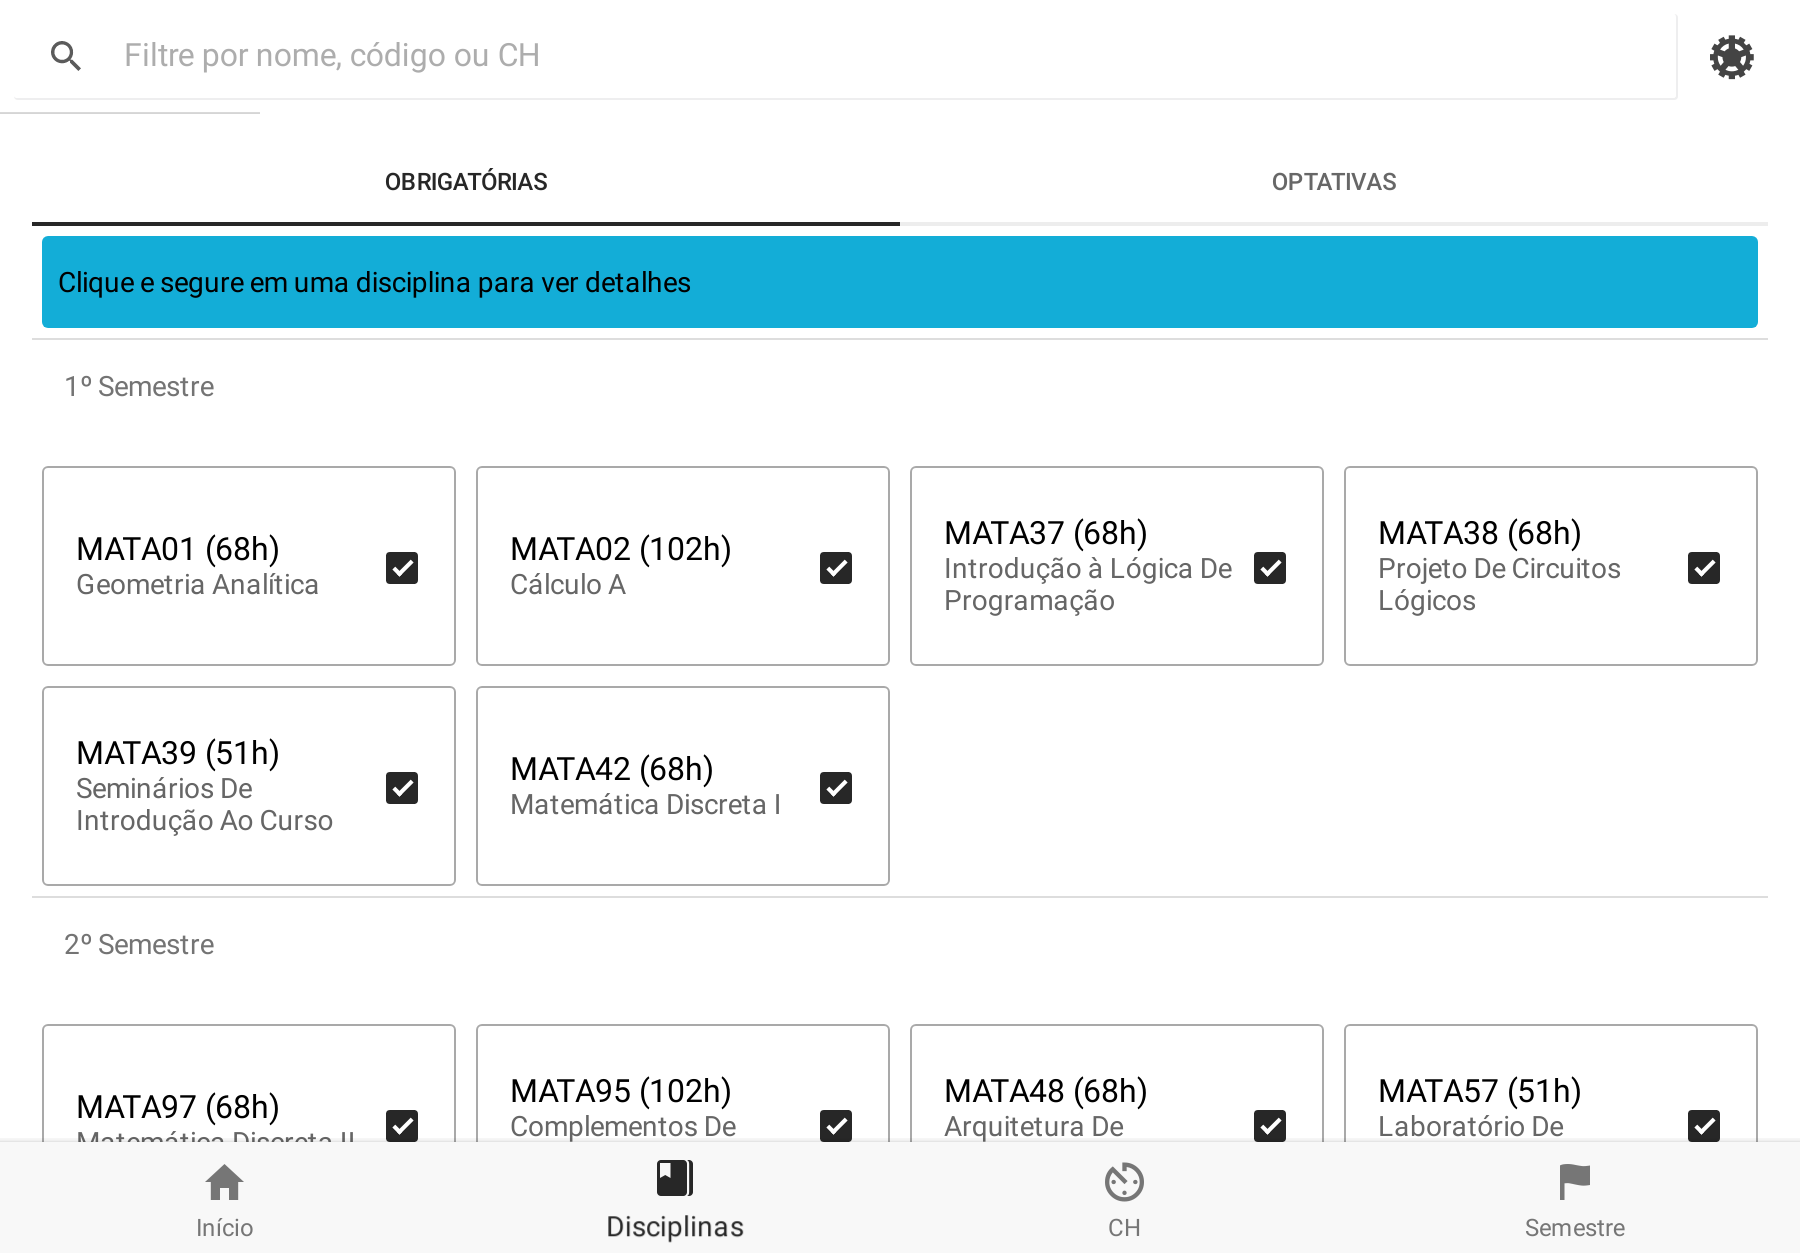
\includegraphics[scale=0.25]{pics/c3/5-disciplines.png}
	   \caption{Tela de disciplinas do curso.}
	   \label{disciplines}
\end{figure}

As disciplinas obrigatórias são segmentadas por semestre (Figura~\ref{disciplines}), a fim de facilitar a identificação de uma disciplina na lista e orientar o usuário com relação à conclusão de um semestre.
As disciplinas optativas exibidas são aquelas sugeridas pelo curso e são exibidas sem categorização (Figura~\ref{optionals}).

\begin{figure}[H]
	   \centering
	   		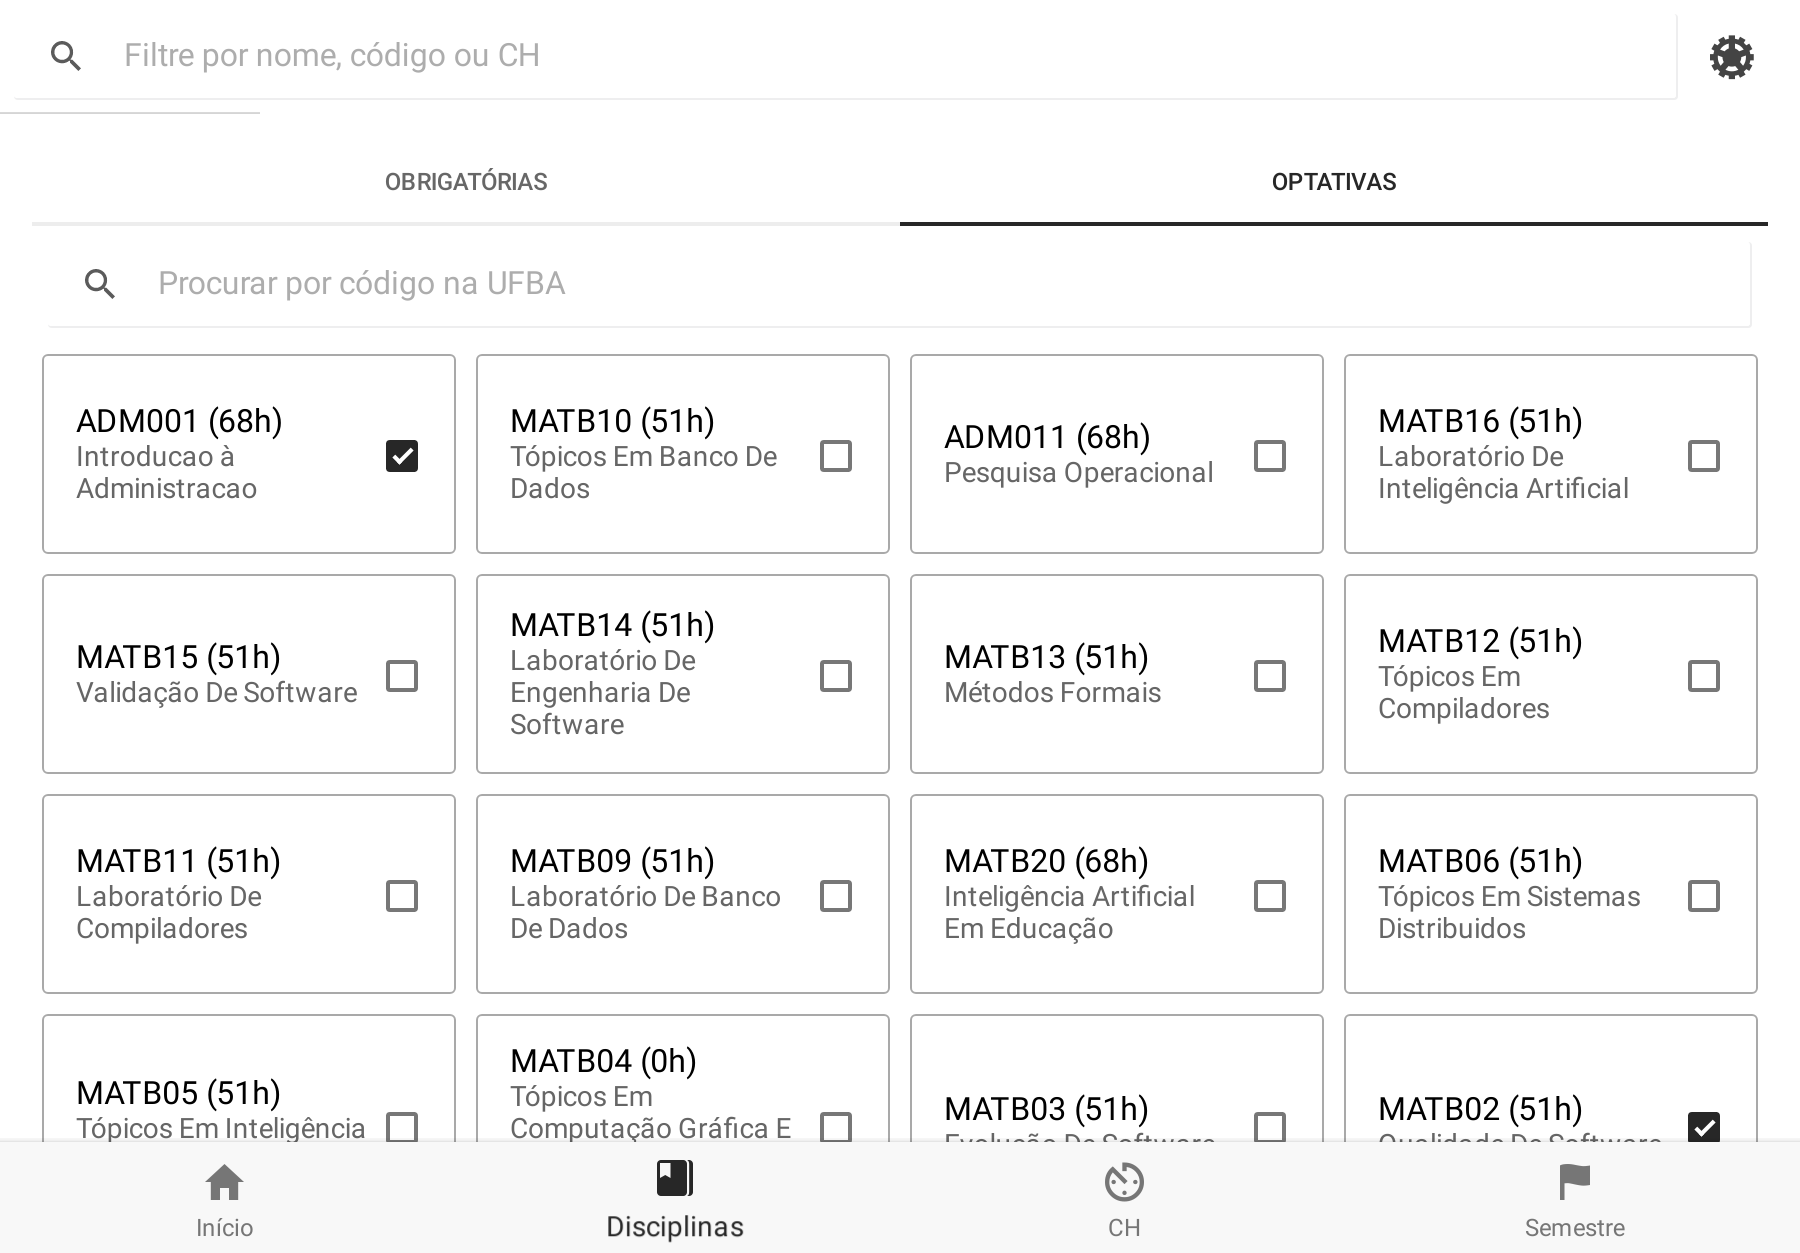
\includegraphics[scale=0.25]{pics/c3/6-optionals.png}
	   \caption{Tela de disciplinas optativas sugeridas pelo curso.}
	   \label{optionals}
\end{figure}

Na seção de disciplinas optativas, o usuário pode buscar uma disciplina em toda a lista de disciplinas do MeForma através do código da disciplina.

O usuário pode ainda buscar uma disciplina por nome, código ou carga horária utilizando a ‘caixa de pesquisa do curso’ localizada no topo da página, mas diferente do campo de busca de optativas, essa caixa de pesquisa só retorna disciplinas que estejam dentre as obrigatórias e optativas oferecidas pelo curso.

Ainda nessa tela, quando o usuário clica e segura em um item, é exibida uma janela no estilo “modal” que exibe a lista completa de pré-requisitos e dependências daquela disciplina.

Na versão web do MeForma, quando o ponteiro do mouse está sob a representação de uma disciplina, os cartões das disciplinas que estão conectadas a ela são destacados. 

A conexão entre disciplinas pode ser do tipo pré-requisito ou do tipo dependência. Sejam A e B duas disciplinas. Se a disciplina A é pré-requisito para a disciplina B, implica que a disciplina B tem a disciplina A como dependência. Graficamente, se uma disciplina A é pré-requisito para uma disciplina B, a disciplina B é destacada na cor verde quando o ponteiro do mouse está sob a disciplina A, por outro lado, quando o ponteiro do mouse está sob a disciplina B, a disciplina A é destacada em tons de vermelho. A Figura~\ref{highlight} mostra a interação do usuário com a disciplina MATA40, que provoca o destaque da disciplina MATA42 como pré-requisito e da disciplina MATA49 como dependente.

O destaque dos pré-requisitos e dependências por cor, tem a finalidade de orientar o usuário com relação à evolução do curso conforme as disciplinas são concluídas.

\begin{figure}[H]
	   \centering
	   		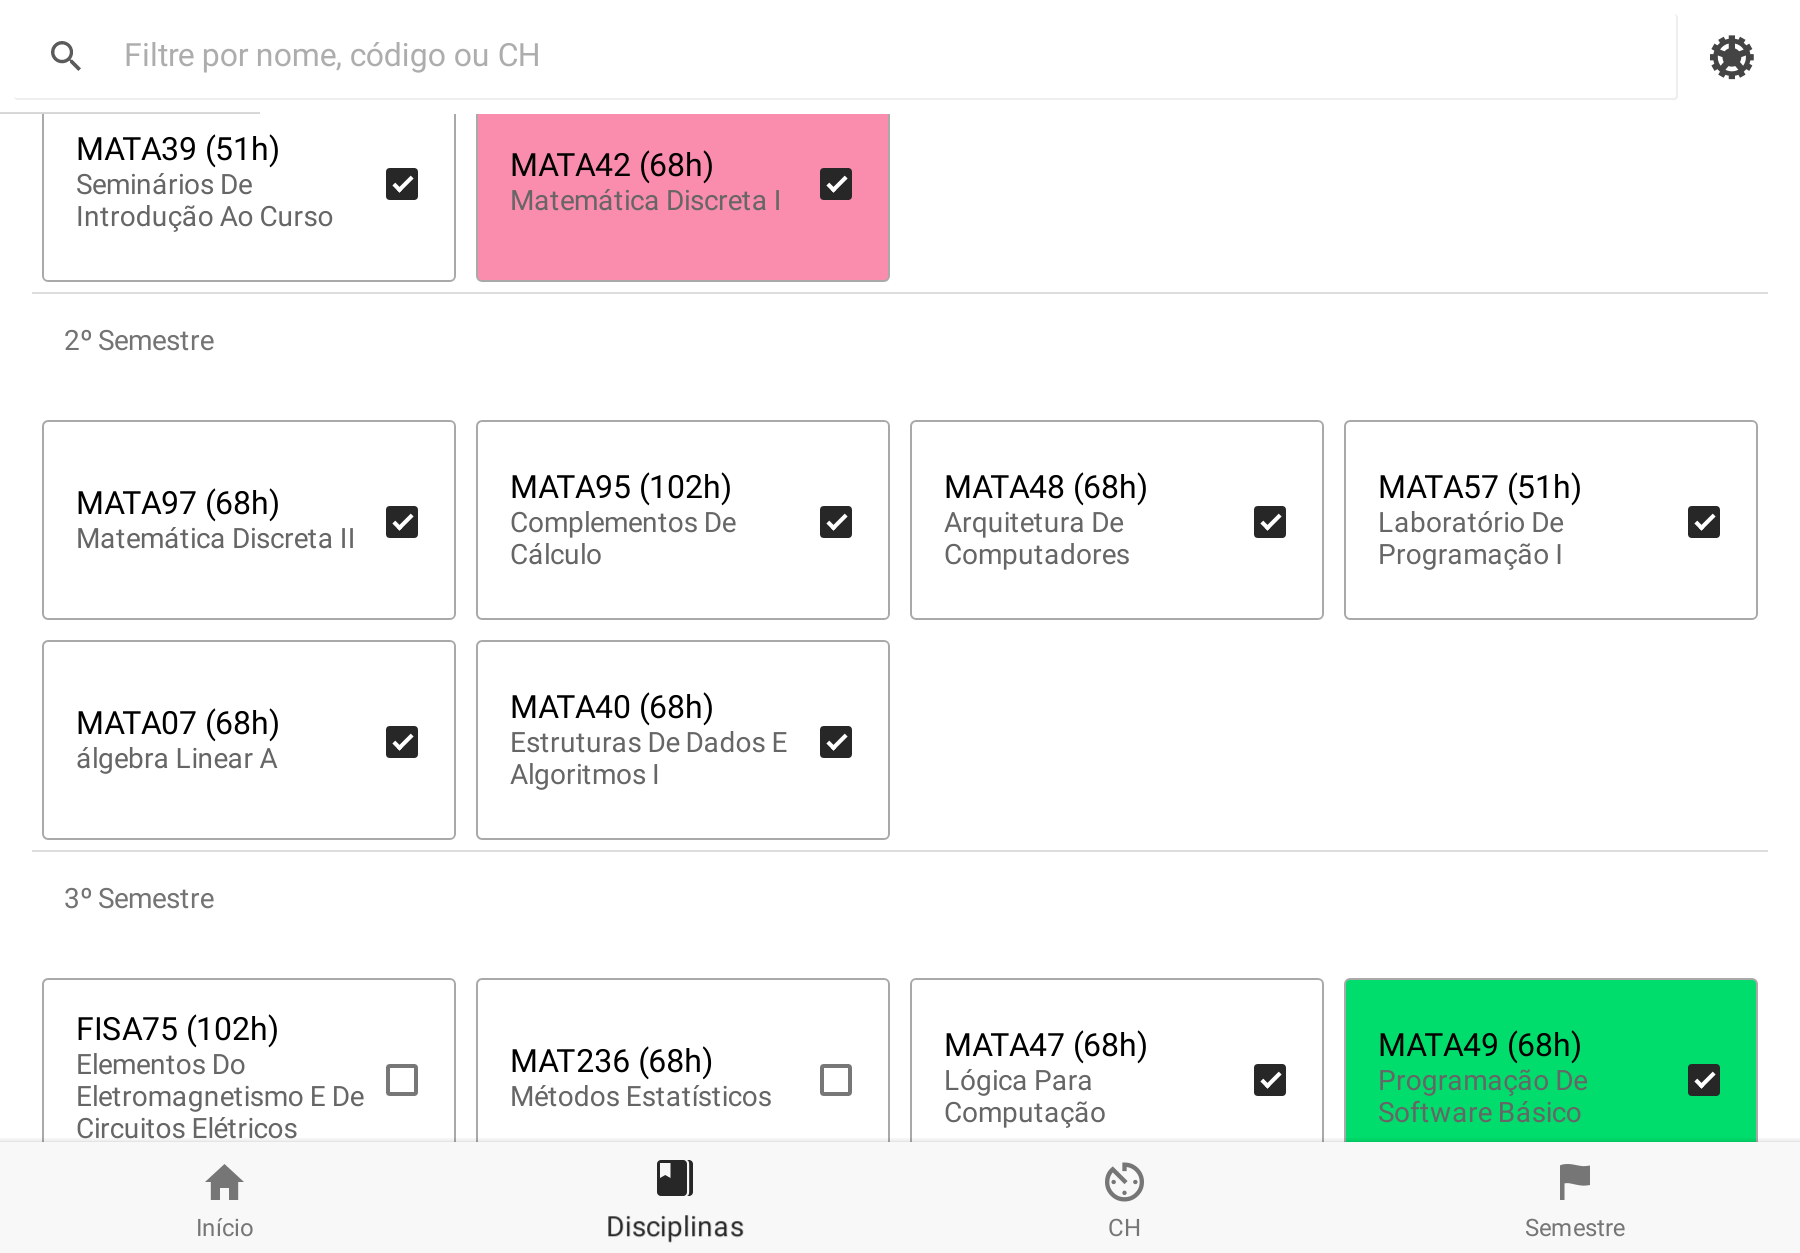
\includegraphics[scale=0.25]{pics/c3/7-highlight.png}
	   \caption{Dependências e pré-requisitos em destaque para a disciplina MATA40.}
	   \label{highlight}
\end{figure}
\subsection{Cadastro de Carga Horária Extra}
A carga horária extra possui três classificações distintas no MeForma2. São elas: optativas, complementares e livres. Cada currículo de curso tem um valor mínimo específico para esses tipos de carga horária. Esse valor também pode ser nulo.

Na tela de carga horária, terceira opção no menu do usuário, os aproveitamentos são secionados de acordo com sua classificação (Figura~\ref{ch}). Ao usuário é apresentado um botão de adição que, ao ser clicado, exibe o formulário de registro de carga horária (Figura~\ref{createch}), o qual exige que o usuário insira a quantidade de horas que foi aproveitada, como essas horas foram aproveitadas,  qual o tipo de carga horária a ser aproveitada (optativa, complementar ou livre) e permite que o usuário deixe um comentário sobre aquele aproveitamento. O registro de um aproveitamento de carga horária o inclui automaticamente no cálculo de conclusão de curso.

Os aproveitamentos são representados por um cartão que exibe como o mesmo se deu, a quantidade de horas correspondentes, e o comentário adicionado pelo usuário, além de oferecer ao usuário as opção de editar e de excluir o aproveitamento. As opções de editar e excluir servem como ferramentas para que os usuários possam se recuperar de erros.

\begin{figure}[H]
	   \centering
	   		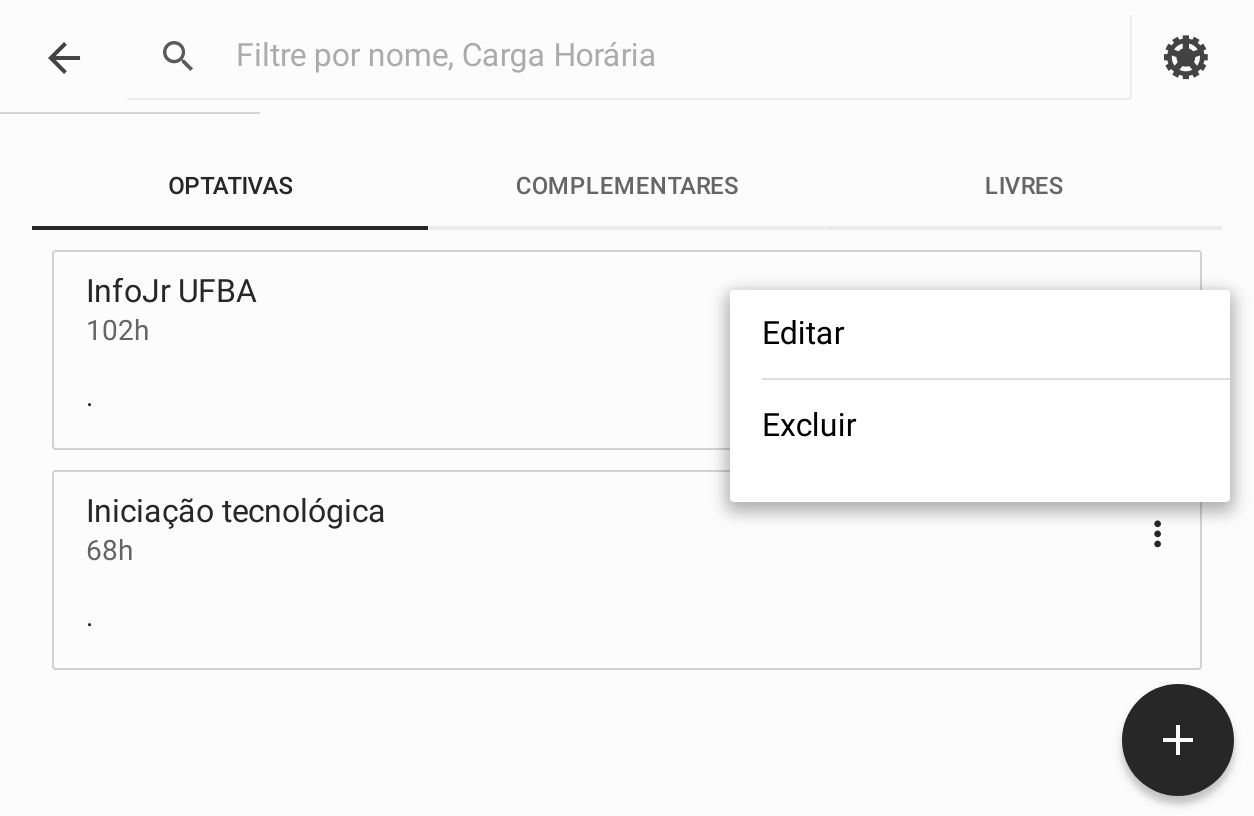
\includegraphics[scale=0.25]{pics/c3/8-ch.png}
	   \caption{Tela de exibição de carga horária.}
	   \label{ch}
\end{figure}

\begin{figure}[H]
	   \centering
	   		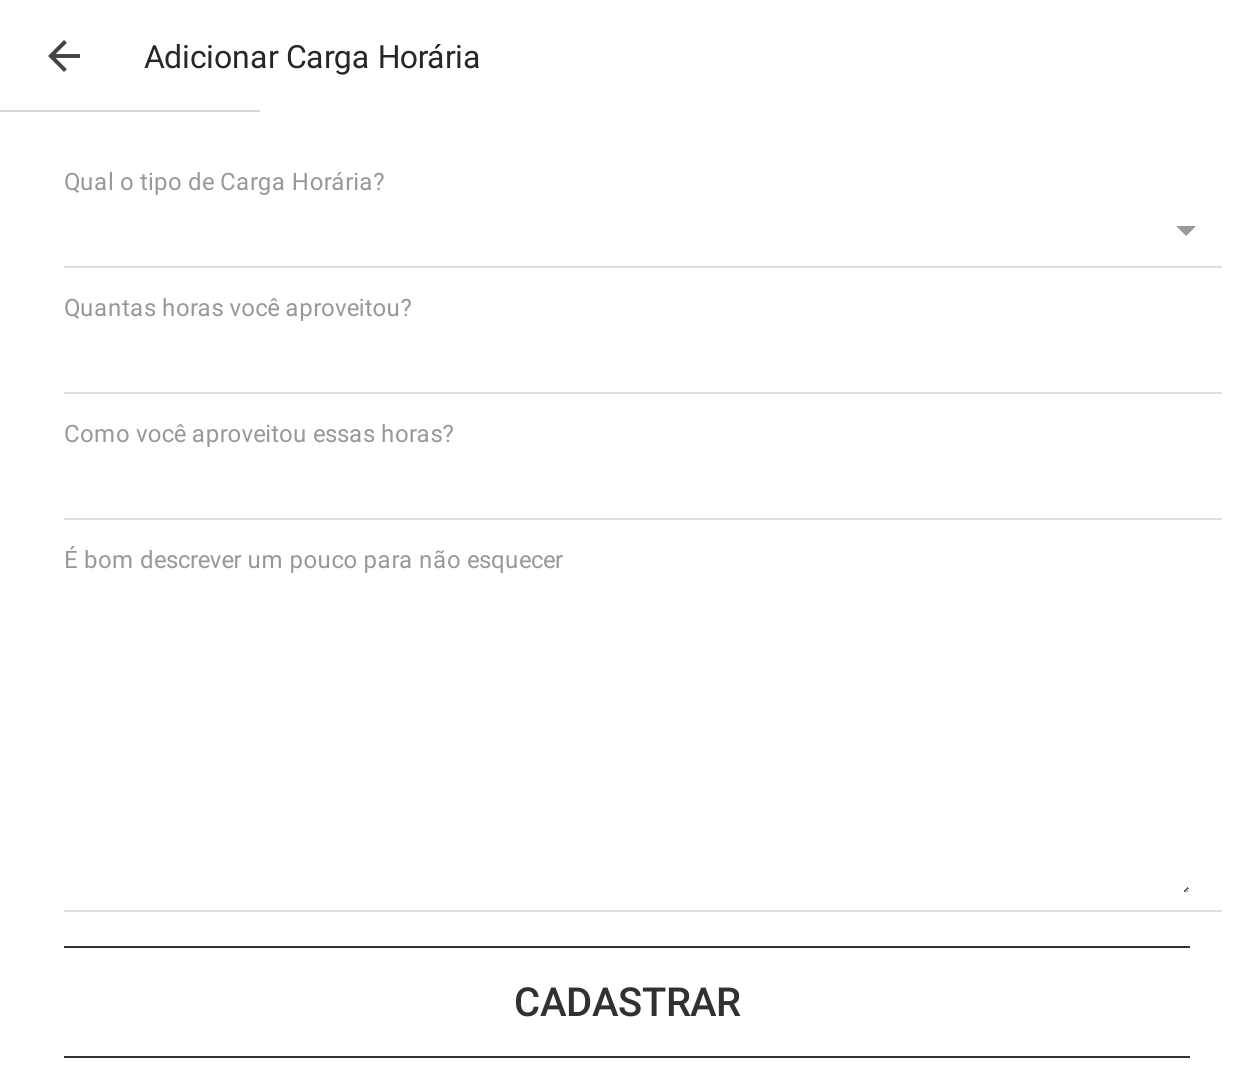
\includegraphics[scale=0.25]{pics/c3/9-createch.png}
	   \caption{Tela de criação de carga horária.}
	   \label{createch}
\end{figure}

\subsection{Registro de Semestre}
O registro de semestre é importante para que o usuário possa controlar seu número de faltas em uma disciplina, além de permitir que ele acompanhe seu avanço no curso. 

O primeiro contato que o usuário tem com os semestres é quando ele acessa a quarta opção do menu do usuário, ``Semestre''. A tela de semestre exibe o semestre mais recente que o usuário registrou e as disciplinas que compõem aquele semestre e, para cada disciplina, o painel de controle de faltas. A tela também exibe as opções de ver todos os semestres e de cadastrar um novo semestre (Figura~\ref{semester}).
\begin{figure}[H]
	   \centering
	   		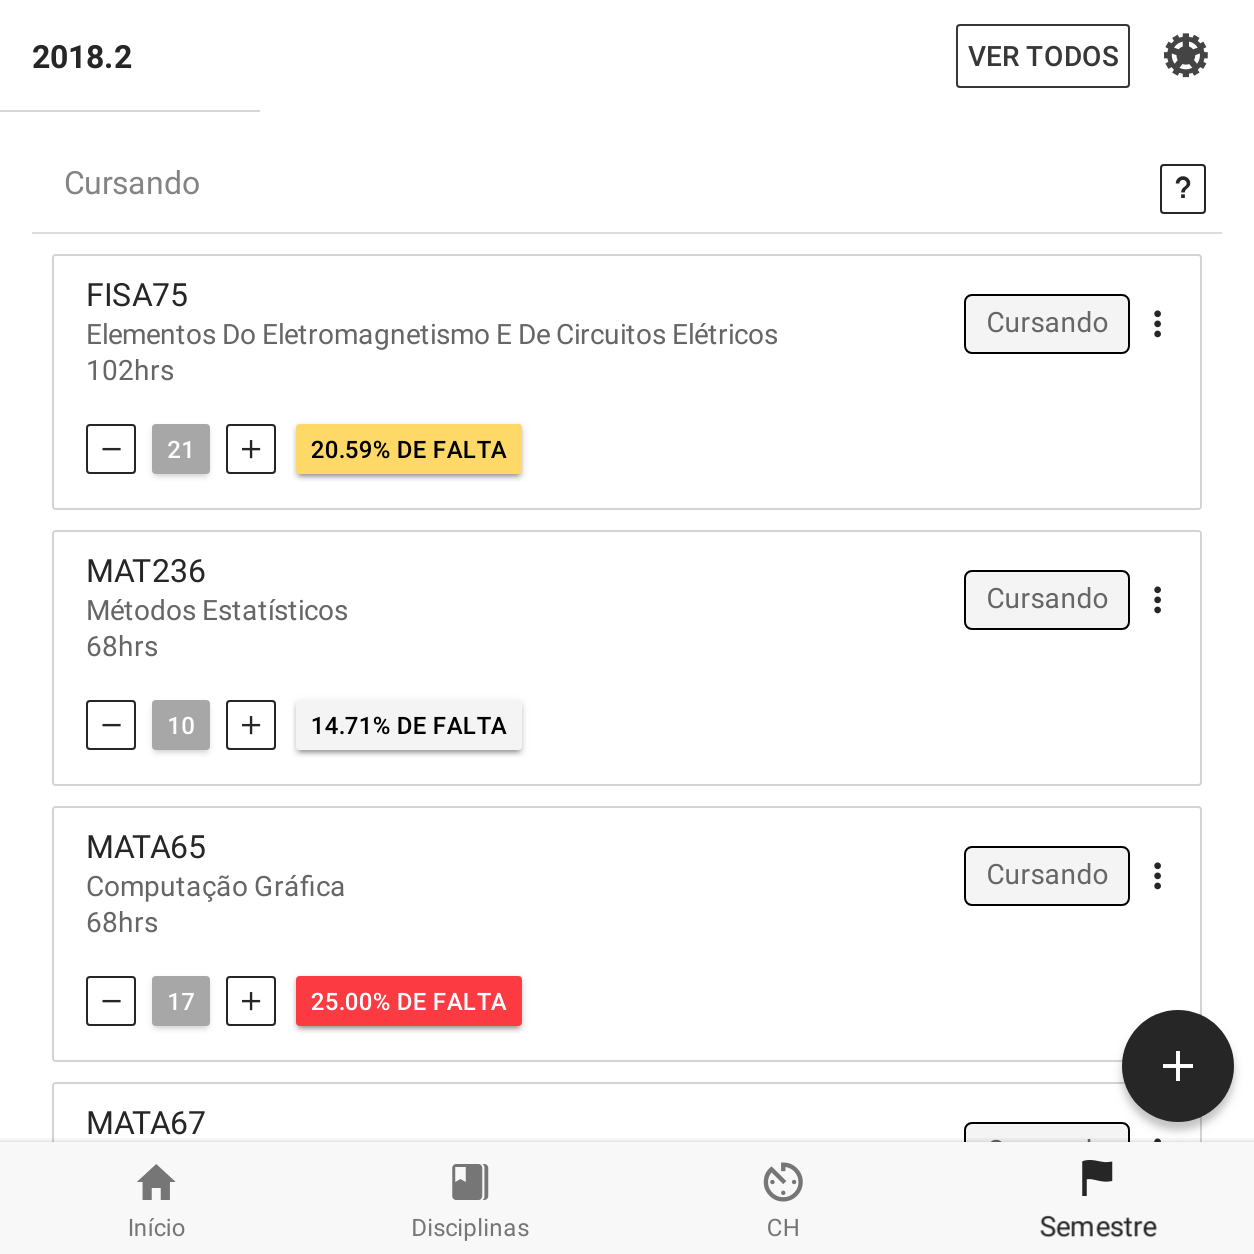
\includegraphics[scale=0.25]{pics/c3/10-semester.png}
	   \caption{Tela de exibição de semestre.}
	   \label{semester}
\end{figure}

A opção de cadastrar um novo semestre exibe uma tela que solicita o código de identificação do semestre que o usuário deseja cadastrar , o qual, após ser inserido, libera a lista de disciplinas do curso para que o usuário possa selecionar as que correspondem àquele semestre (Figura~\ref{newsemester}.

\begin{figure}[H]
	   \centering
	   		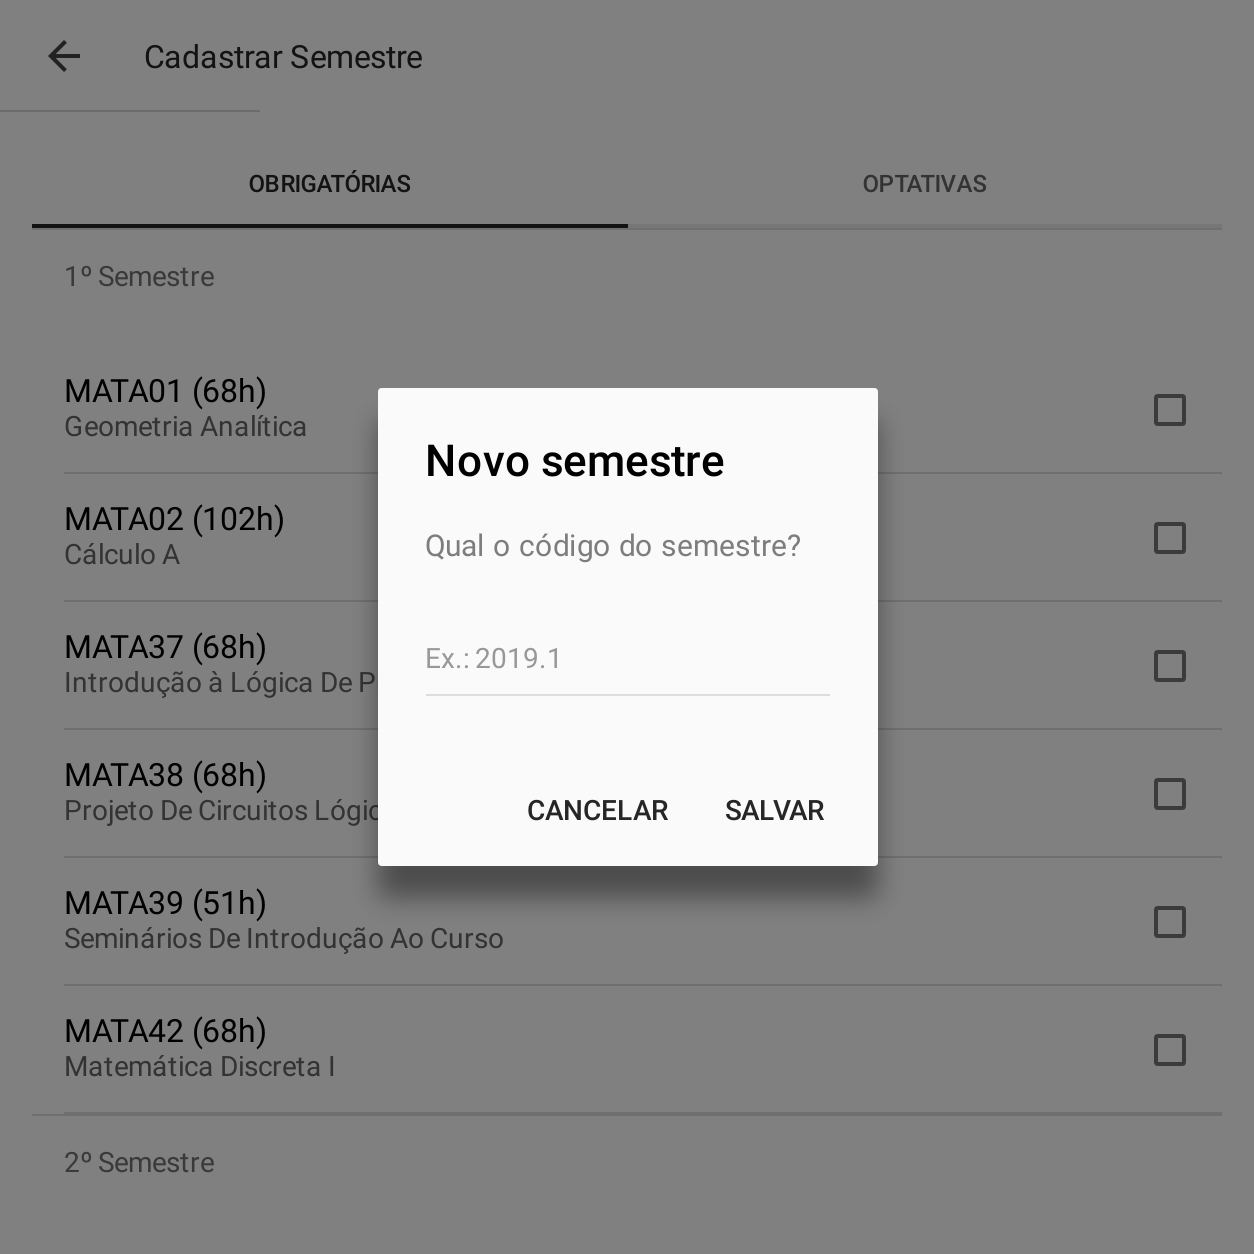
\includegraphics[scale=0.25]{pics/c3/11-newsemester.png}
	   \caption{Tela de cadastro de semestre.}
	   \label{newsemester}
\end{figure}

A opção ``Ver Todos'' exibe uma lista com todos os semestres cadastrados no sistema pelo usuário e as opções de editar um semestre (que implica na possibilidade de alterar o código de identificação), alterar disciplinas, e excluir semestre.

Nas telas de ``Semestre atual'' e de ``Todos os semestres'', cada disciplina é apresentada graficamente como um cartão que oferece ao usuário dois botões responsáveis por incrementar e decrementar as faltas naquela disciplina. As faltas são alteráveis em qualquer tempo. A funcionalidade de controle de faltas é exibida na figura~\ref{semester}.

\subsection{Recuperação de Dados do Siac Web}
O Siac é um portal onde os estudantes da UFBA podem acompanhar dados referentes à matrícula semestral. Através desse portal o MeForma é capaz de obter automaticamente os dados sobre as disciplinas optativas e obrigatórias cursadas pelo estudante necessários para o gráfico de conclusão. A Figura \ref{siac} mostra como o estudante pode recuperar os dados do Siac.

\begin{figure}[H]
	   \centering
	   		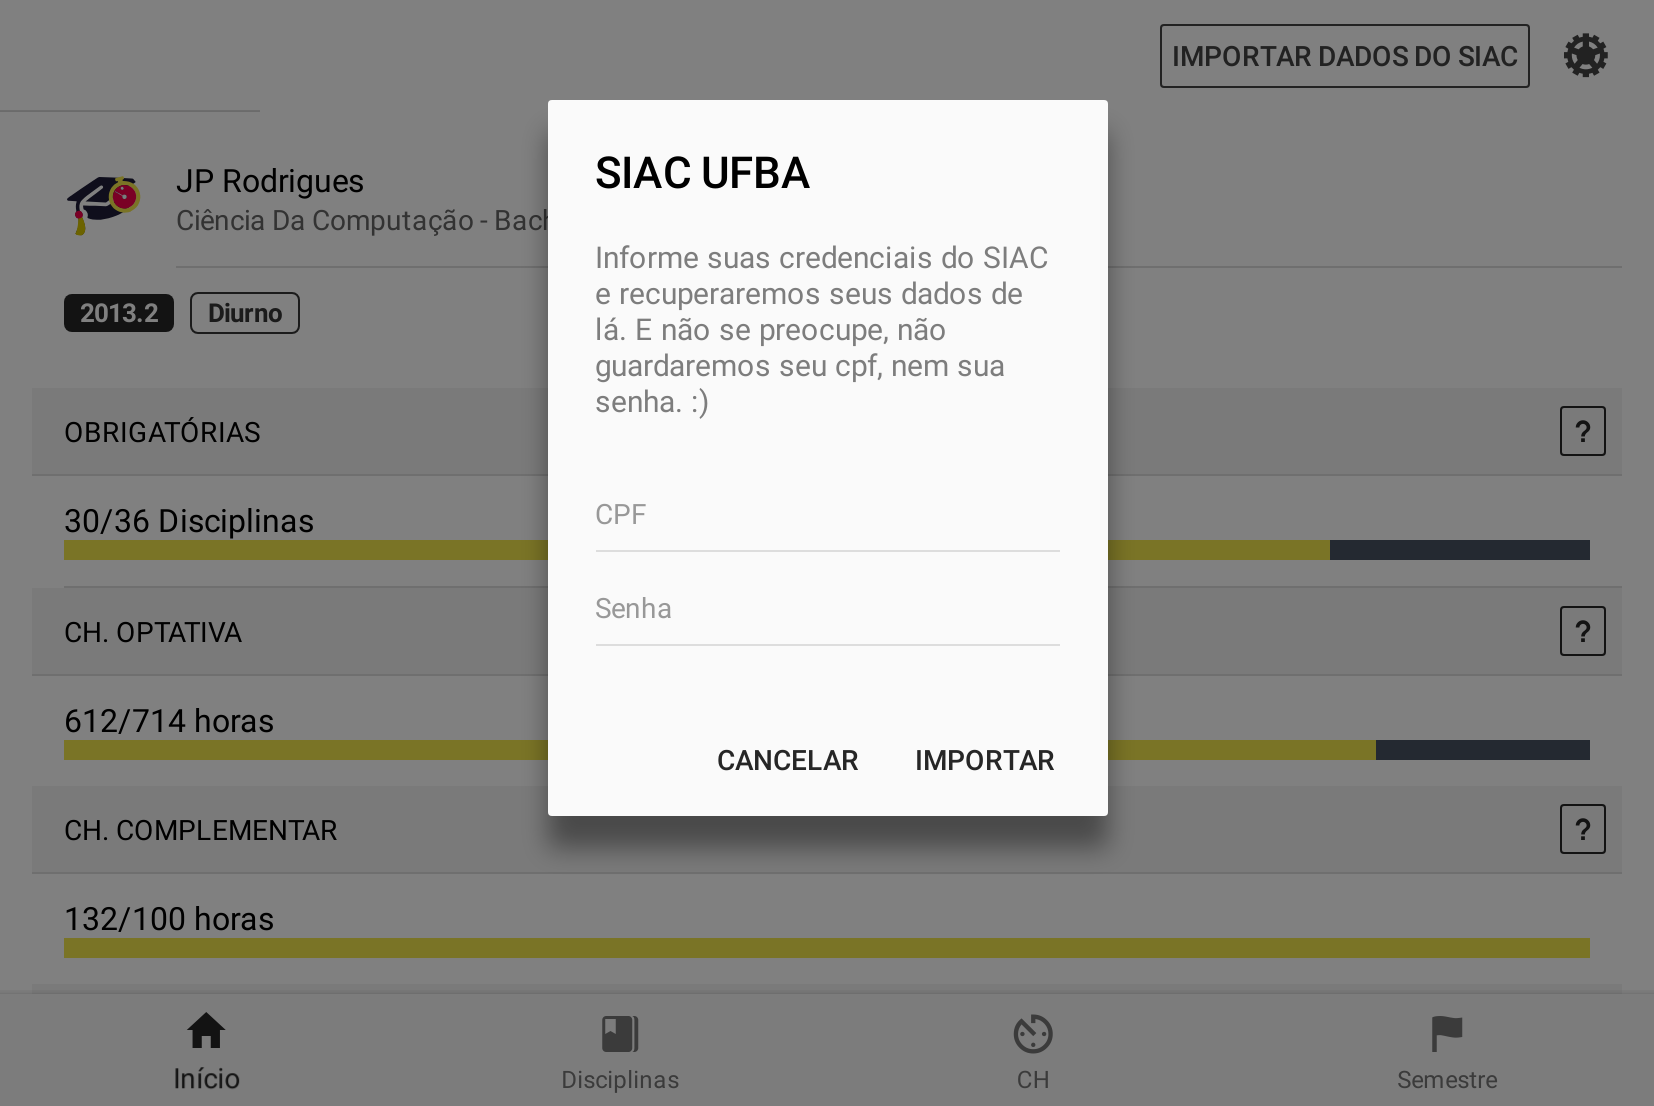
\includegraphics[scale=0.25]{pics/c3/13-siac.png}
	   \caption{Tela de recuperação de dados do Siac.}
	   \label{siac}
\end{figure}

\subsection{Porcentagem de aprovação das disciplinas}

Quando o estudante recupera seus dados do Siac, a tela de disciplinas do curso passa a exibir a porcentagem de aprovação de cada disciplina, a fim de ajudar o estudante a planejar o conjunto de disciplinas que ele vai cursar por semestre.

A porcentagem de aprovação é acompanhada por uma barra de status que indica através das cores vermelho, amarelo e azul a categoria da disciplina com relação à porcentagem de aprovações. A cor vermelho indica um número criticamente baixo de aprovações, a cor amarelo indica um número baixo de aprovações, a cor azul indica um número satisfatório de aprovações. A Figura \ref{percentages} exibe a tela de disciplinas do curso com as suas respectivas porcentagens de aprovação.

O cálculo de porcentagem de aprovação considera apenas os estudantes cadastrados no MeForma2 que estão cursando o mesmo currículo de curso que o usuário que está acessando o sistema e que recuperaram seus dados do Siac. Esses limites foram impostos para aumentar a confiabilidade dos números gerados.

Um detalhe importante sobre a porcentagem de aprovação é que ela diz respeito à amostra de estudantes que estão cadastrados no MeForma2, desse modo, para que o valor seja próximo da realidade do currículo do curso, o ideal é que muitos estudantes tenham recuperado seus dados do Siac.


\begin{figure}[H]
	   \centering
	   		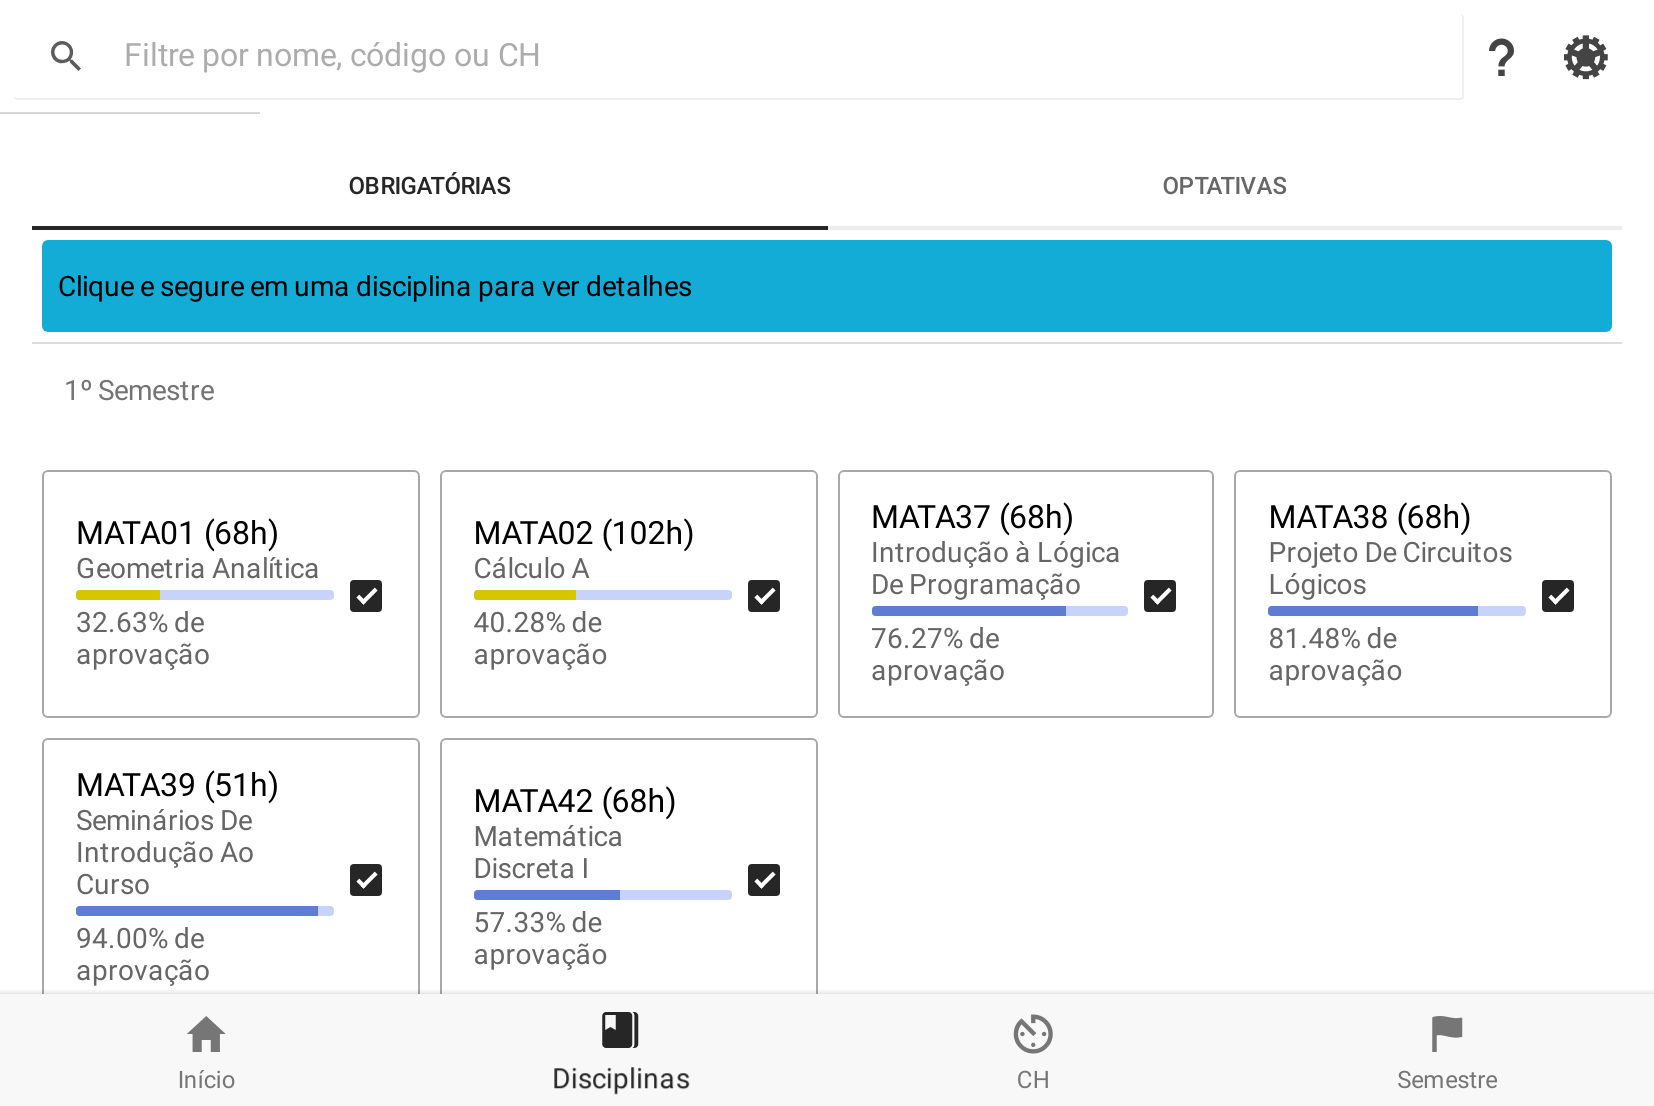
\includegraphics[scale=0.25]{pics/c3/14-percentage.png}
	   \caption{Tela de disciplinas do curso com porcentagem de aprovação.}
	   \label{percentages}
\end{figure}

\section{Painel de Acompanhamento dos Cursos}

O Painel de Acompanhamento dos Cursos - MFPAC é uma sequência de telas do MeForma2 disponível apenas para gestores dos cursos de graduação cadastrados no sistema. Com o MFPAC o gestor pode analisar os dados gerados pela utilização do MeForma2 por parte dos estudantes de cada currículo dos cursos que ele gerencia. A seguir serão apresentadas as principais telas que compõem o painel.

\subsection{Resumo de desempenho nas disciplinas}

A tela de resumo de desempenho das disciplinas exibe 5 gráficos que apresentam as 10 disciplinas com maior porcentagem de aprovação, as 10 disciplinas com maior porcentagem de reprovação, as 10 disciplinas com maior porcentagem de desistência, as 10 disciplinas com maior porcentagem de trancamento e as 10 disciplinas com maior porcentagem de reprovações por falta. Os dados podem ser filtrados por curso, currículo e período. A Figura \ref{charts} exibe a tela de resumo de desempenho das disciplinas para o curso de Ciência da Computação da UFBA referentes aos estudantes com currículo 2013.2 para o período de 2010.2 a 2018.2.

As porcentagens são calculadas apenas com os estudantes que recuperaram seus dados do Siac, a fim de melhorar a confiabilidade dos números. Contudo, vale ressaltar que os números são referentes a uma amostra que se aproxima dos valores reais conforme aumenta a quantidade de estudantes cadastrados no MeForma2.

\begin{figure}[H]
	   \centering
	   		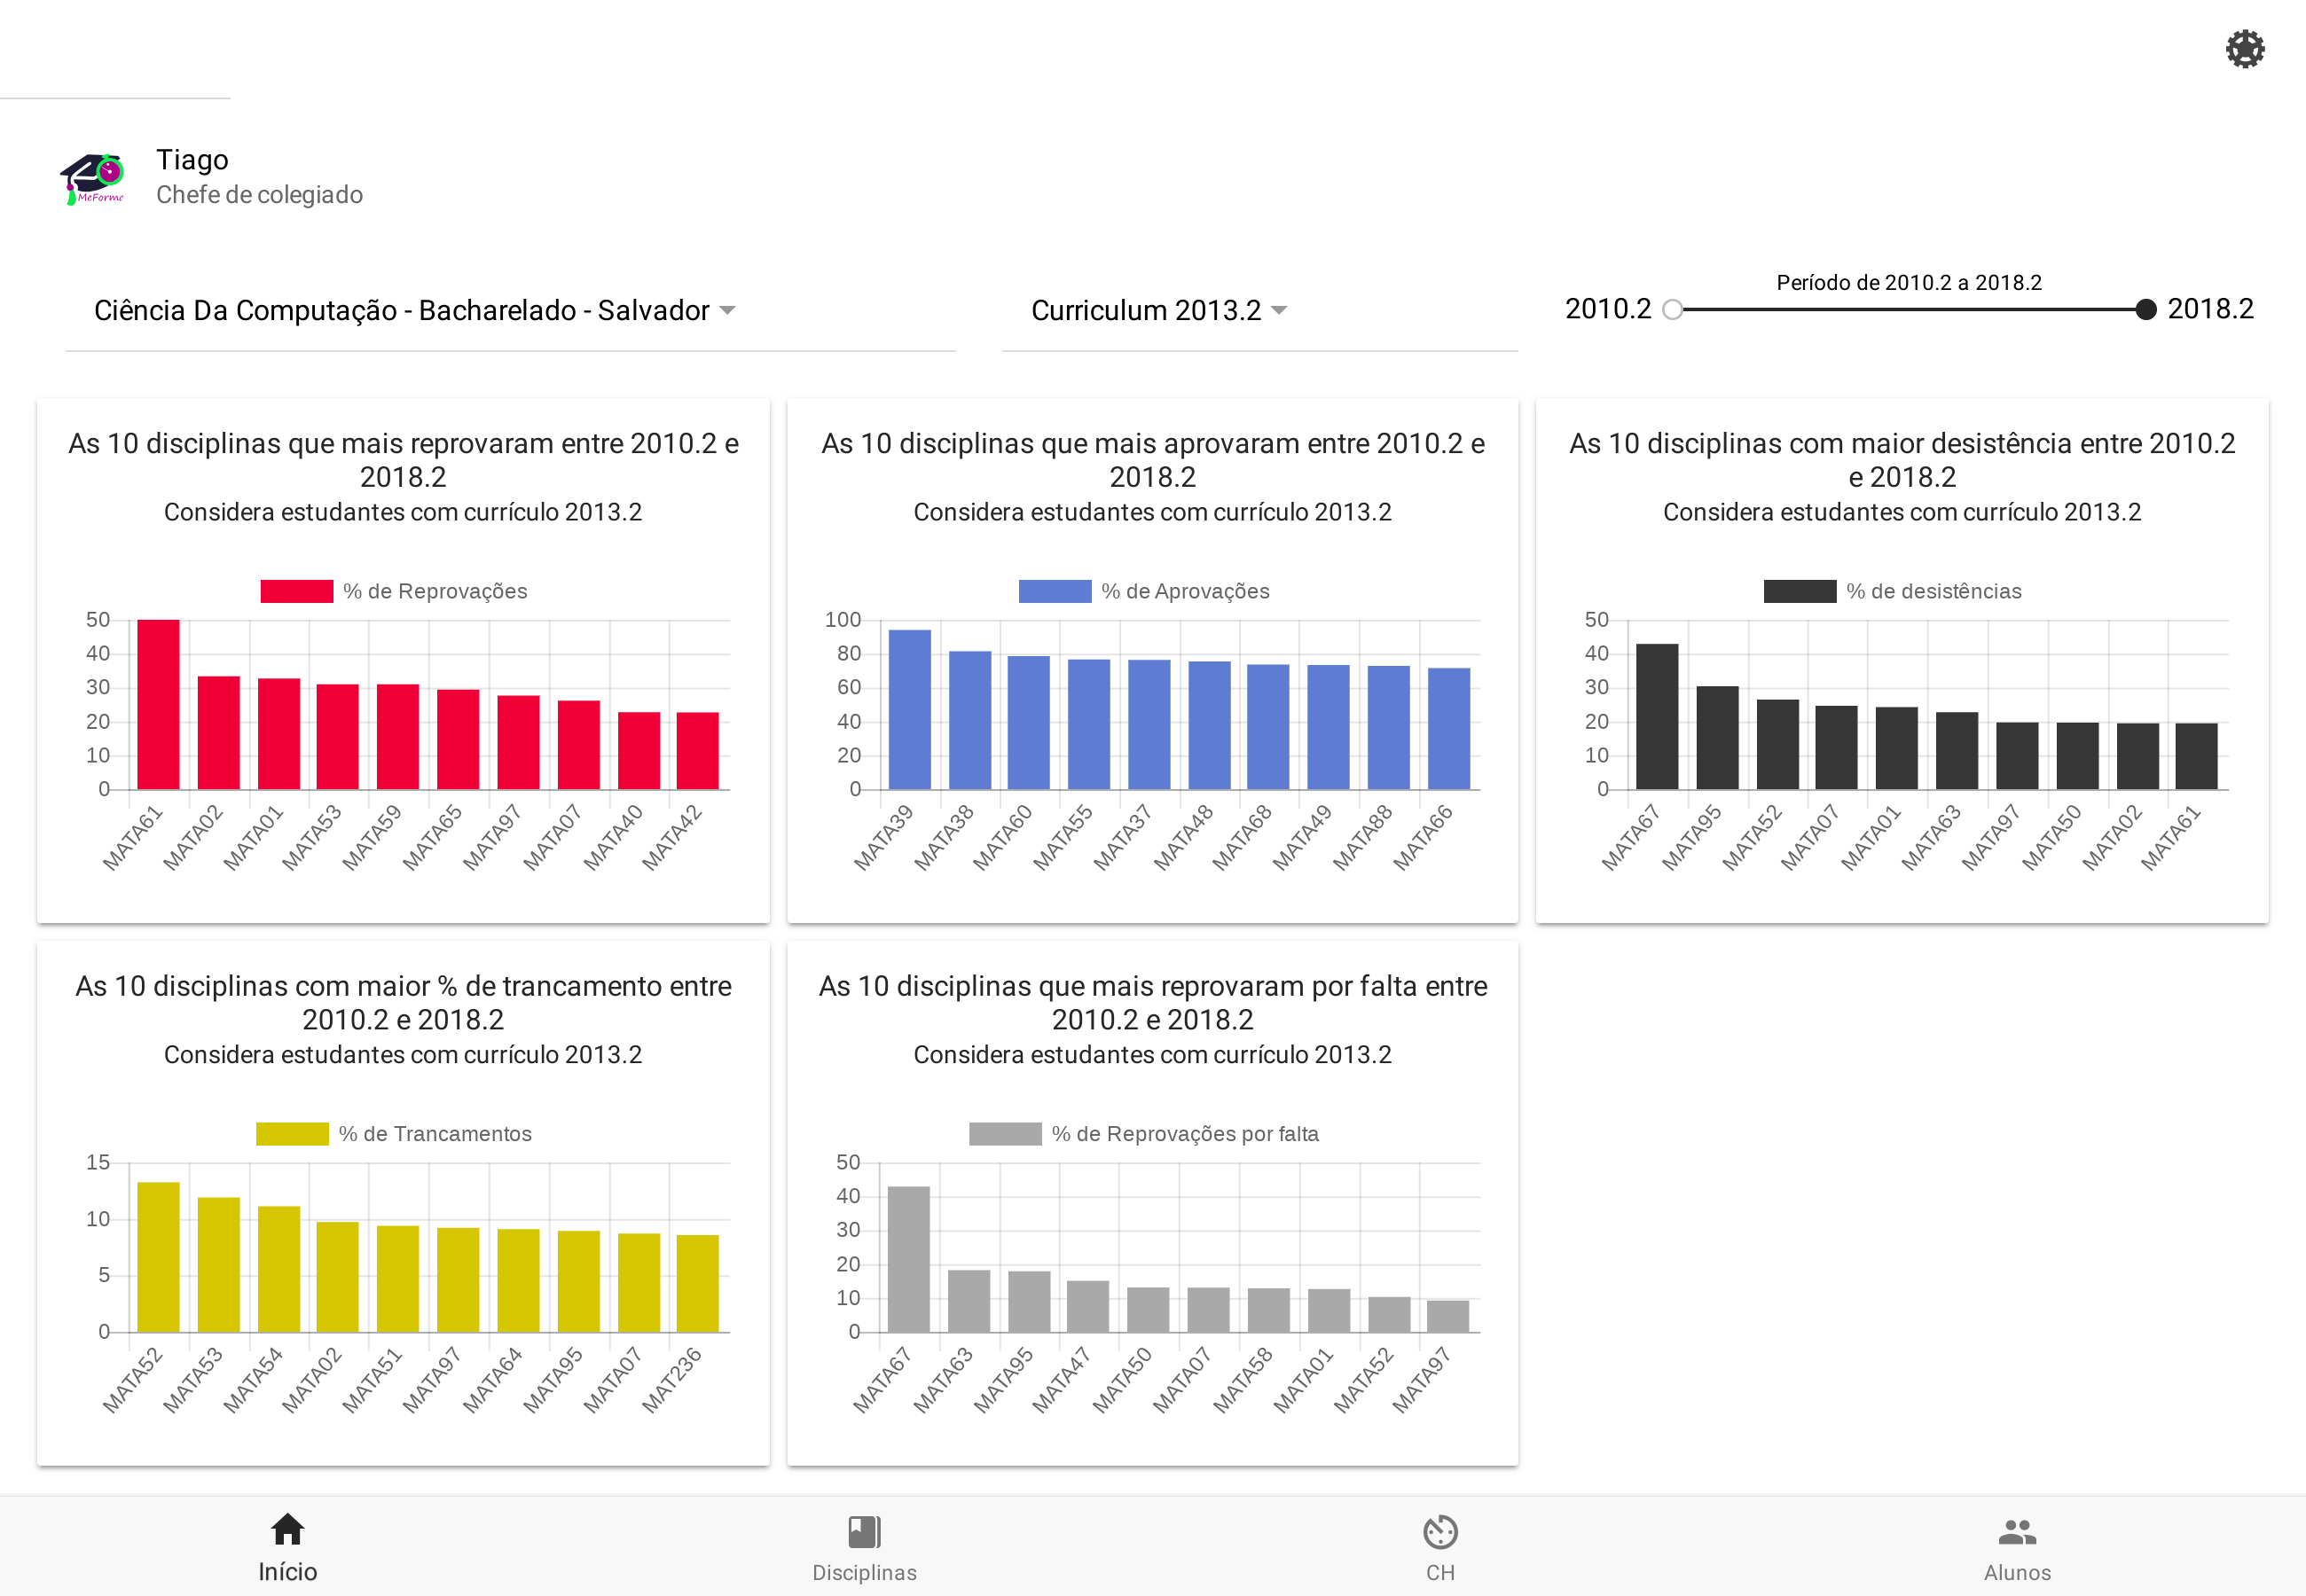
\includegraphics[scale=0.15]{pics/c3/15-charts.png}
	   \caption{Tela de resumo de desempenho nas disciplinas.}
	   \label{charts}
\end{figure}

\subsection{Lista de disciplinas do curso}

A tela de disciplinas do curso é semelhante em aparência àquela descrita na subsessão \ref{disciplinas_tela}, contudo, no MFPAC o objetivo é acompanhar o desempenho geral dos estudantes de um dado currículo em cada disciplina no decorrer do tempo. Para tal, além da porcentagem de aprovação de cada disciplina, quando o usuário clica em um cartão de disciplina, é exibido um gráfico que compara os percentuais de aprovação, reprovação, desistência, trancamento e reprovação por falta daquela disciplina. A Figura \ref{discipline-chart} exibe o desempenho dos estudantes do curso de Ciência da Computação da UFBA com currículo 2013.2 para o período de 2010.2 a 2018.2 na disciplina ``Compiladores''.

\begin{figure}[H]
	   \centering
	   		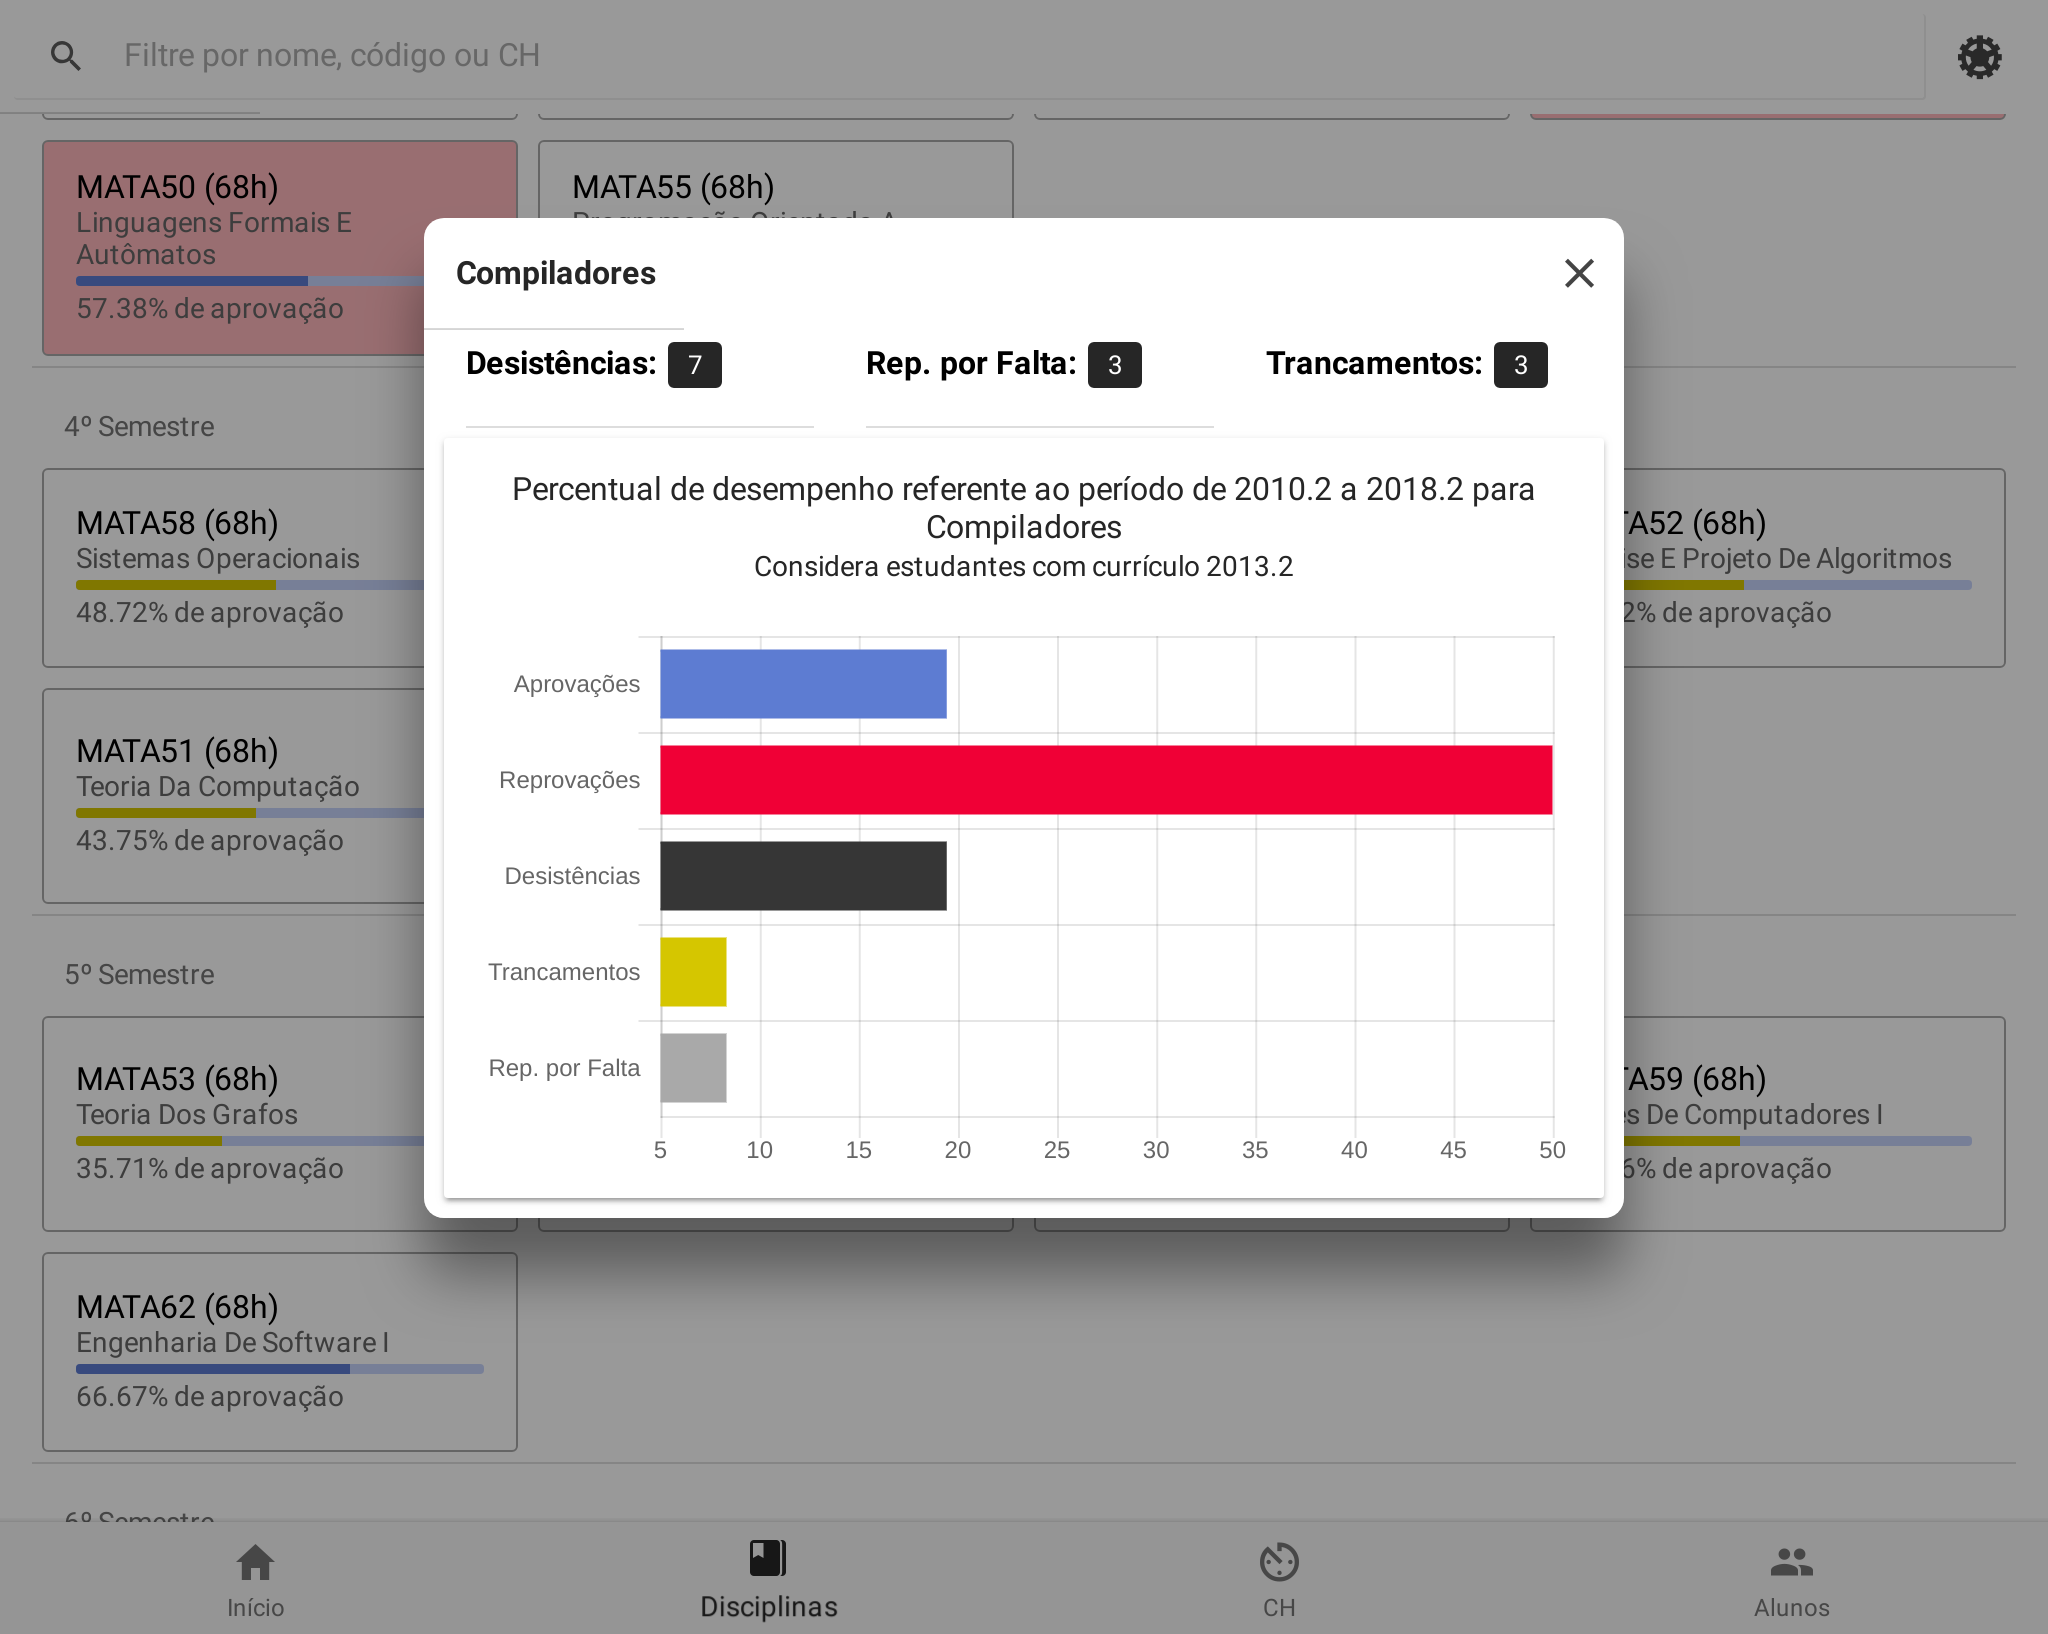
\includegraphics[scale=0.15]{pics/c3/16-compiladores.png}
	   \caption{Dados sobre a disciplina Compiladores.}
	   \label{discipline-chart}
\end{figure}

\subsection{Aproveitamentos de carga horária}

O objetivo dessa tela é exibir como os estudantes tem aproveitado carga horária para que o gestor possa principalmente dar indicações a alunos que precisam de carga horária. A Figura \ref{pacch} exibe a tela de aproveitamentos de carga horária.

\begin{figure}[H]
	   \centering
	   		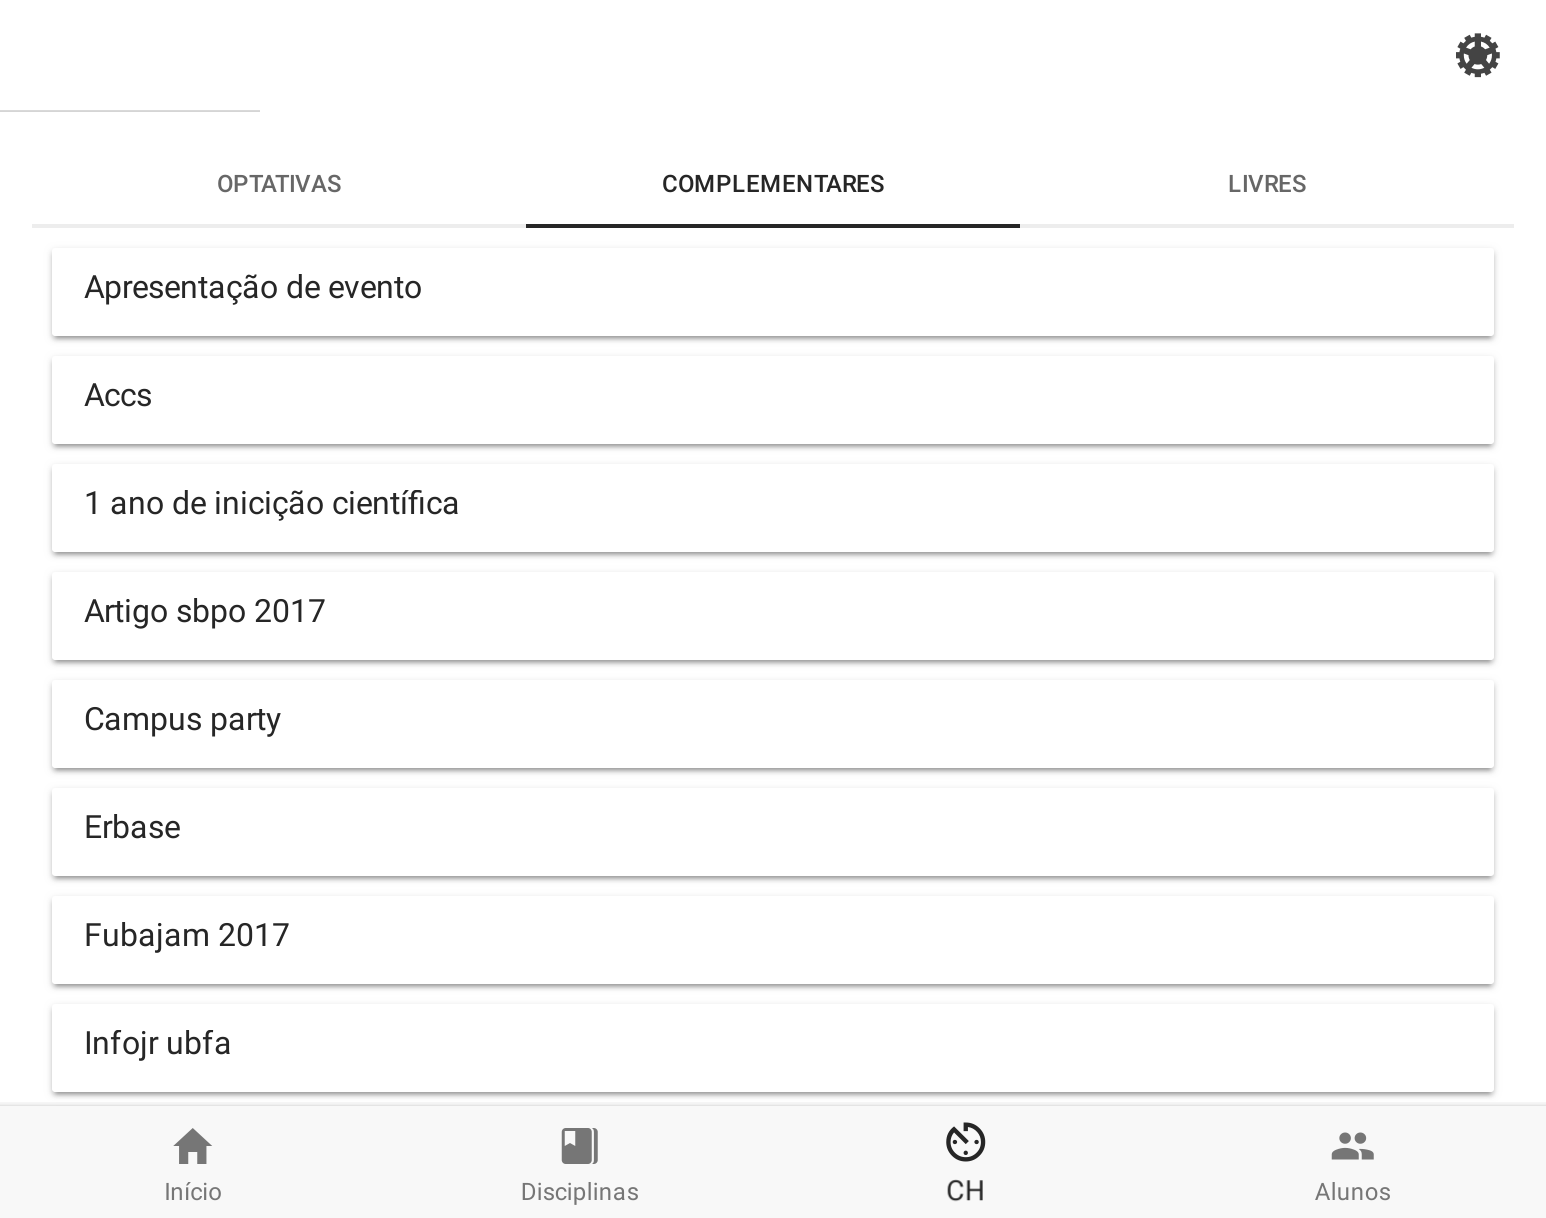
\includegraphics[scale=0.25]{pics/c3/17-ch.png}
	   \caption{Tela de aproveitamentos de carga horária.}
	   \label{pacch}
\end{figure}

\subsection{Listagem de estudantes}

A tela de listagem de estudantes tem o objetivo de exibir os estudantes que estão cadastrados no MeForma2 e os dados de curso dos mesmos, fornecendo ao gestor a quantidade de disciplinas que o estudante já cumpriu, a quantidade de carga horária que ele já proveitou e a quantidade mínima de semestres necessários para o estudante alcançar a formatura.

A quantidade mínima de semestres necessários para um estudante alcançar a formatura é calculada com base nas disciplinas obrigatórias que o mesmo ainda não cumpriu. Os demais requisitos para completude de um curso não foram incluídos no cálculo, pois a quantidade de horas que um aluno pode aproveitar em um semestre é imprevisível. A seguir é apresentado o algoritmo utilizado para determinar esse número.

\begin{enumerate}
    \item Subtrai-se o conjunto de disciplinas obrigatórias cursadas do conjunto de disciplinas obrigatórias total para obter o conjunto de disciplinas não cursadas.
    \item Contrói-se um grafo com as disciplinas não cursadas, onde cada disciplina é um vértice, a dependência entre elas são as arestas e o subgrafo formado por uma disciplina e suas dependências é uma árvore cuja altura determina a quantidade de semestres necessários para cumprir todas as disciplinas da árvore.
    \item A altura de cada árvore de disciplina é calculada e o valor da maior delas é armazenado.
    \item A moda da quantidade de disciplinas encaixadas em cada semestre do currículo do curso é calculada.
    \item A quantidade de disciplinas restantes é dividida pela moda calculada no passo 4 e armazenada.
    \item A quantidade de semestre necessários para cumprir as disciplinas obrigatórias restantes é dada pelo maior número entre o obtido no passo 3 e o obtido no passo 5.
\end{enumerate}

A Figura \ref{dgraph} exibe um grafo montado conforme o passo 2 para um usuário que precisa cumprir apenas as disciplinas MATA01, MATA02, MATA07, MATA65, MATA236 e FISA75. A maior altura de uma árvore para esse grafo é três (passo 3), e assumindo que a moda da quantidade de disciplinas por semestre é seis (passo 4), e como sete dividido por seis é menor do que três, a quantidade mínima de semestres necessárias para o aluno cumprir tais disciplinas é três. 

\begin{figure}[H]
	   \centering
	   		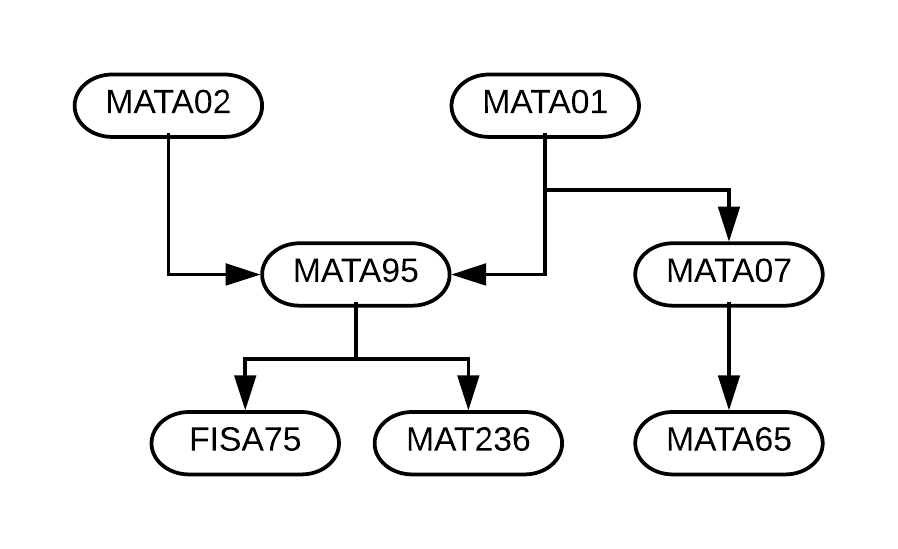
\includegraphics[scale=1.3]{pics/c3/19-graph.png}
	   \caption{Grafo de dependência entre as disciplinas restantes.}
	   \label{dgraph}
\end{figure}


A Figura \ref{students} exibe a tela de listagem de estudantes. Os dados pessoais que identificam o estudante foram propositalmente escondidos.  

\begin{figure}[H]
	   \centering
	   		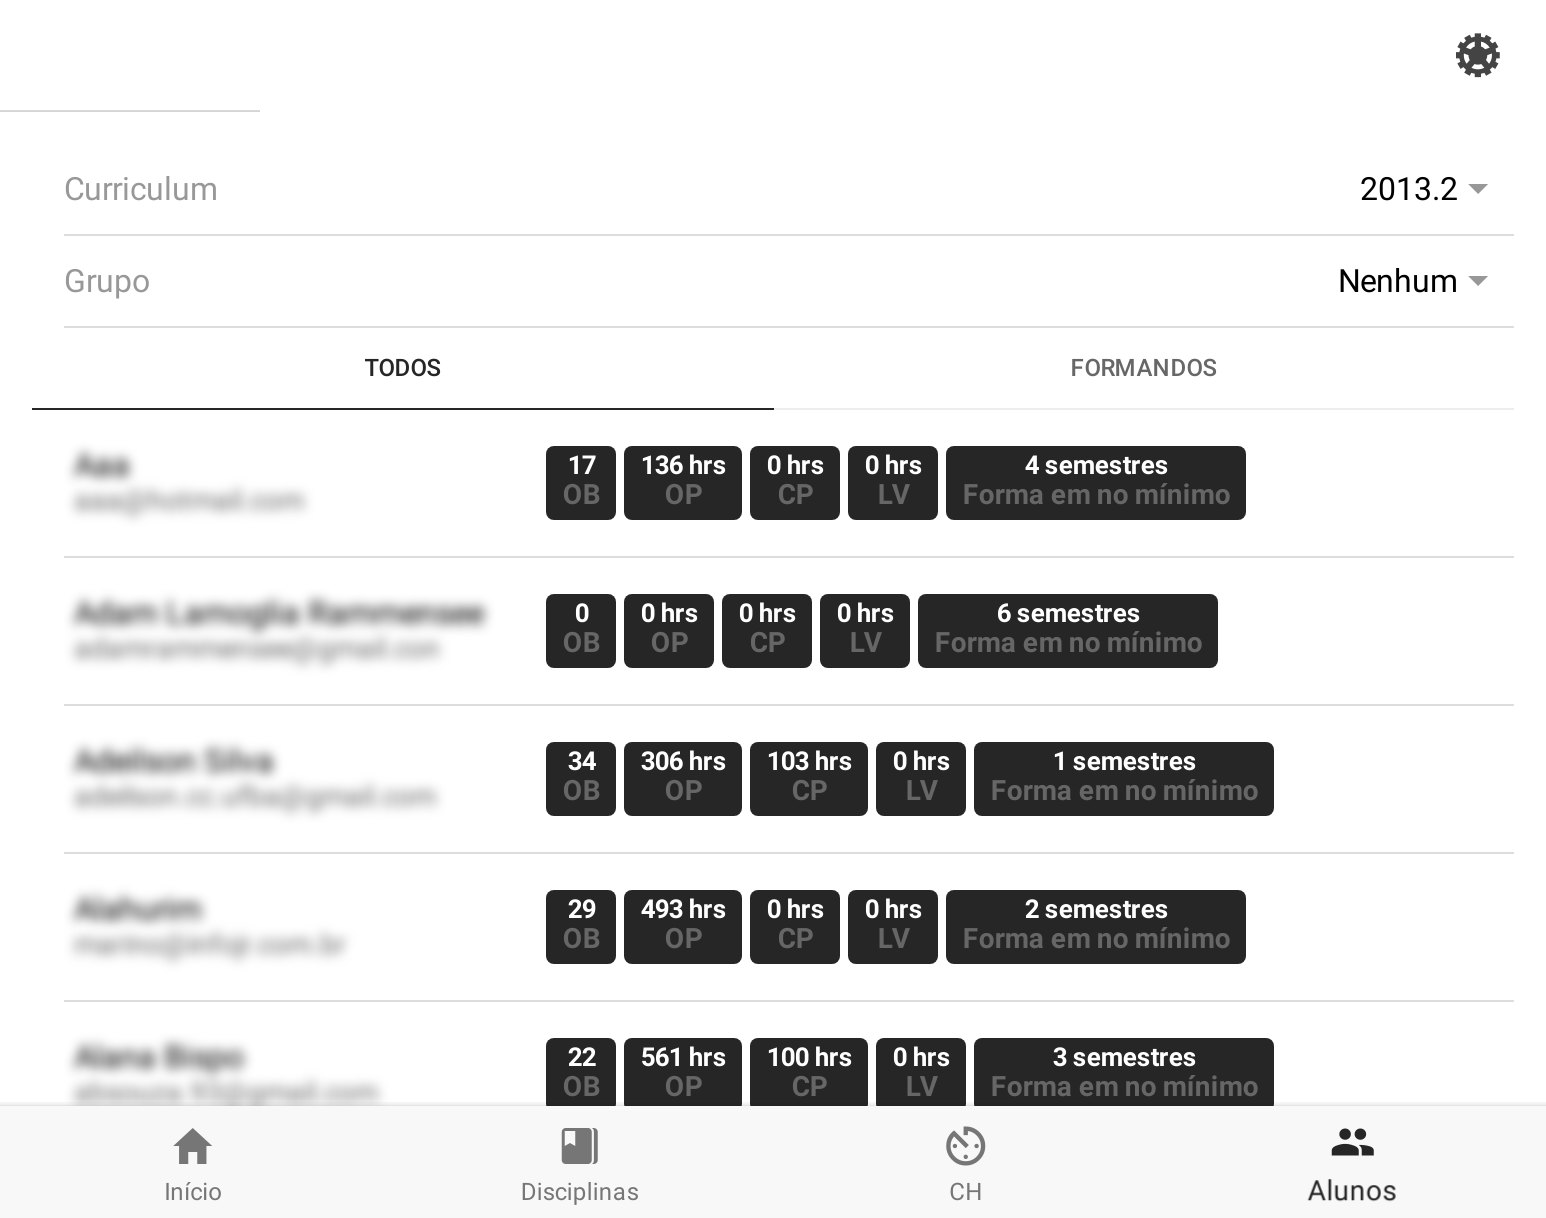
\includegraphics[scale=0.25]{pics/c3/18-students.png}
	   \caption{Tela de listagem de estudantes.}
	   \label{students}
\end{figure}


\section{Arquitetura do Aplicativo}
\label{frontend}
A seguir será apresentada a arquitetura do aplicativo, e a relação de comunicação entre as tecnologias que a compõem. Considerando como ponto de partida as tecnologias que estão em contato com o usuário, tecnicamente chamadas de ``Tecnologias FrontEnd'' até as tecnologias que estão funcionando em segundo plano no dispositivo do usuário.

\begin{figure}[H]
	   \centering
	   		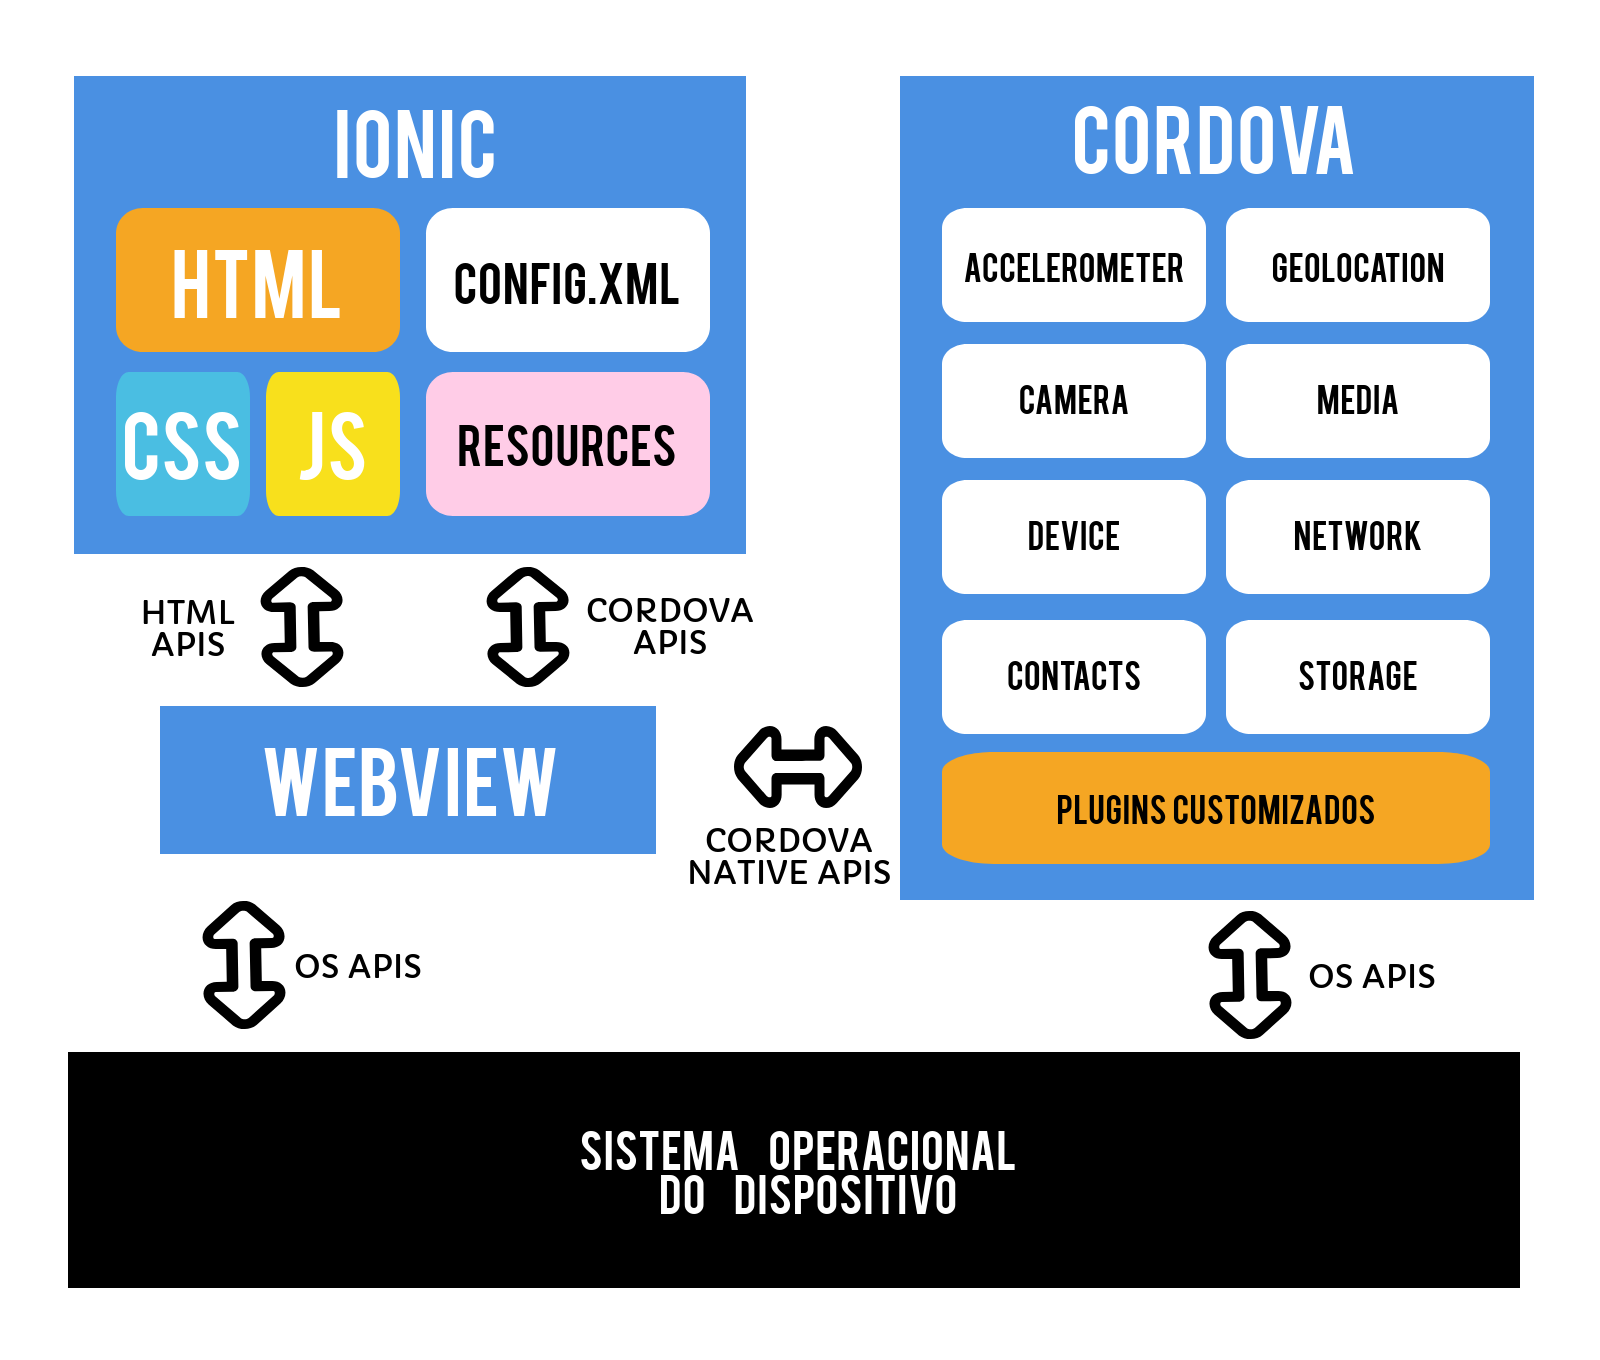
\includegraphics[scale=0.28]{pics/c3/0-arquitetura.png}
	   \caption{Arquitetura do Aplicativo}
	   \label{arquitetura}
\end{figure}

A figura~\ref{arquitetura} mostra a relação entre os componentes do aplicativo do MeForma2. Cada uma das caixas mais externas representa uma tecnologia. Cada seta na figura representa uma ponte de comunicação entre as tecnologias.

\section{Ionic Framework}

Com o Ionic Framework, ou simplismente Ionic, foi produzido o código fonte do aplicativo. Esse código fonte é dividido em 5 categorias de arquivos: HTML, CSS, JS, config.xml, e os resources que, no caso do MeForma são as imagens locais. Os arquivos HTML, CSS e JS são gerados após os pré-processadores cidatos na Seção~\ref{tecnologias} serem executados pelo Ionic.

O aplicativo é implementado como uma página da Web. Por padrão, um arquivo local chamado index.html faz referência ao CSS, JavaScript, imagens e outros recursos necessários para sua execução. O aplicativo é renderizado em um \textit{WebView} através da ponte de comunicação \textit{HTML APIs}.

Esse pacote tem ainda um arquivo config.xml que fornece informações sobre o aplicativo e especifica parâmetros que afetam como ele funciona, por exemplo, se o aplicativo deve responder às mudanças de orientação do dispositivo.

\subsection{WebView}

O \textit{WebView} é um componente do sistema operacional dos dispositivos móveis modernos para quando se quer entregar um aplicativo da Web como um aplicativo mobile ou como parte de um aplicativo. Seu funcionamento é semelhante ao de um navegador da Web, porém ele não inclui nenhum recurso de um navegador da Web totalmente desenvolvido, como controles de navegação ou uma barra de endereços. O que o WebView faz, por padrão, é executar e exibir uma página da web.

O WebView é capaz de estabelecer uma comunicação entre o conteúdo gerado pelo Ionic e o Cordova. E, quando a aplicação é executada num navegador da Web, é ele quem faz o papel do WebView.

\subsection{Cordova}

O Cordova é responsável por envolver o aplicativo em um contêiner com acesso às funções nativas do dispositivo em que o aplicativo está sendo executado. Essas funções são exposta via JavaScript para facilitar a integração com o aplicativo e com o WebView.

No código gerado pelo Ionic deve haver a informação de quais plugins do Cordova serão utilizados e de como deve ser essa utilização, então isso é solicitado do \textit{WebView} (Cordova APIs) que, por sua vez, solicita do Cordova (Cordova Native Apis).

\subsection{Sistema Operacional do Dispositivo}

O sistema operacional do dispositivo é o provedor dos recursos necessários para que o WebView e o Cordova possam utilizar o hardware do dispositivo do usuário.

\section{Arquitetura Lógica da Aplicação}

Esta seção descreve a arquitetura lógica do MeForma2. A aplicação foi desenvolvida utilizando o padrão de arquitetura de software \textit{Model–view–controller} (MVC). No MVC, o sistema é estruturado em três componentes lógicos que interagem entre si: Model, Controller e View.

\begin{itemize}
    \item O Model é o componente responsável pelo gerenciamento dos dados do sistema. Ele é o componente mais próximo do SGBD e seu papel no MeForma2 é realizar operações de leitura, atualização, criação e exclusão de dados.
    \item O Controller é o componente responsável pelas regras de negócio da aplicação e realiza tarefas de controle e tratamento de informações e dados.
    \item A View é o componente que define como as informações são apresentadas ao usuário.
\end{itemize}
\begin{figure}[H]
	   \centering
	   		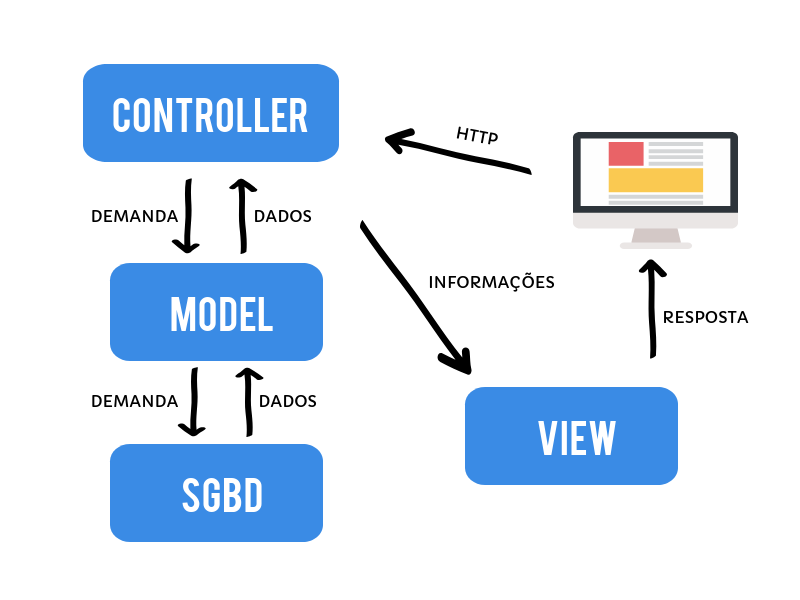
\includegraphics[scale=0.50]{pics/c3/12-mvc.png}
	   \caption{Representação conceitual do padrão MVC.}
	   \label{mvc}
\end{figure}
A Figura~\ref{mvc} mostra a relação entre os componentes do MVC e a conexão entre o MVC e o usuário (representado por um computador) que também pode ser interpretado como sendo o aplicativo. O usuário solicita um recurso do sistema através de uma requisição HTTP (padrão de comunicação utilizado na web), essa requisição é interpretada pelo Controller que a encapsula como uma demanda para o Model. Este, por sua vez, converte a demanda para um modelo de demanda do SGBD. O SGBD encaminha ao Model os dados correspondentes à demanda que recebeu, então o Model transforma os dados para um modelo que o Controller possa interpretar e os encaminha para ele. O Controller interpreta os dados recebidos do Model e os organiza para gerar informações, as quais são enviadas ao View que as padroniza para que sejam exibidas no dispositivo do usuário.

No MeForma2, os componentes do MVC são agrupados em um modelo de organização característico de aplicativos multiplataforma. Os componentes Controller e Model são agrupados em um pacote denominado API do inglês \textit{Application Programming Interface}.

A API do MeForma2 é responsável pela comunicação entre o aplicativo e o banco de dados. Por um lado, ela é a encarregada de transformar e controlar o conteúdo proveniente do Banco de Dados para que o aplicativo possa interpretar e exibir. No sentido oposto, ela é responsável por transformar os dados inseridos no aplicativo pelo usuário para que possam ser devidamente registrados no banco de dados.

\section{Banco de dados}

Essa seção justifica a estrutura adotada para armazenamento dos dados do MeForma2 em banco de dados.

\begin{figure}[H]
	   \centering
	   		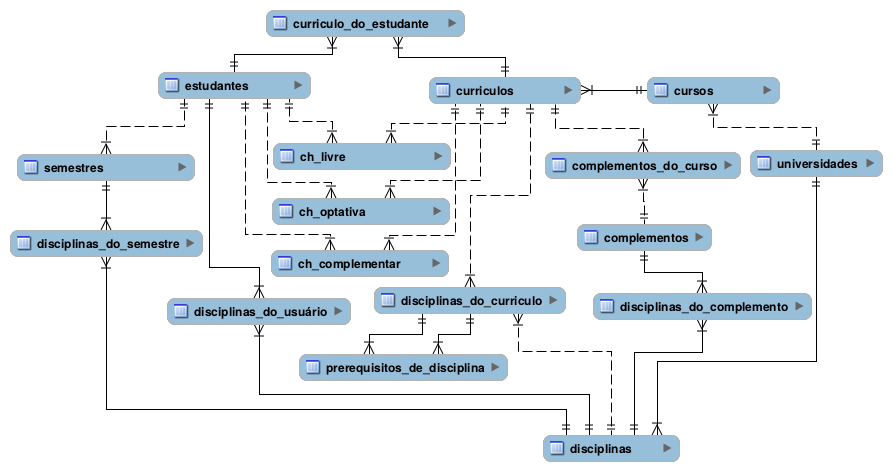
\includegraphics[scale=0.50]{pics/c3/4-db.png}
	   \caption{Diagrama de organização e relacionamento das tabelas}
	   \label{db}
\end{figure}

A Figura~\ref{db} mostra um diagrama de organização do banco de dados do MeForma2. A figura mostra como os dados do MeForma2 estão relacionados na estrutura de armazenamento.

Existem 3 tabelas principais no MeForma: a tabela ``estudantes'', a tabela ``currículos'' e a tabela ``disciplinas''. Elas estão no centro da aplicação e representam a região mais congestionada.

A estrutura pode ainda ser dividida em duas partes, a primeira composta pelas tabelas que dizem respeito aos dados que o sistema fornece ao usuário, que serão chamadas de ``tabelas do sistema'', e a segunda composta pelas tabelas que dizem respeito aos dados que o usuário fornece ao sistema, que serão chamadas de ``tabelas do usuário''.

\subsection{Tabelas do Sistema}
As tabelas que dizem respeito aos dados que o sistema fornece ao usuário são: ``universidades'', ``cursos'', ``currículos'', ``disciplinas'', ``disciplinas\_do\_currículo'', ``prerequisitos\_de\_disciplinas'', ``complementos'', ``complementos\_do\_curso'' e
``disciplinas\_do\_complemento''.

As tabelas ``universidades'' e ``cursos'' funcionam apenas como um filtro para o currículo. Todas as relações posteriores tratam de um estudante em seu currículo de curso ou de um currículo de curso e suas disciplinas.

É o currículo quem determina o tempo máximo e mínimo de formatura, a quantidade de carga horária que um estudante precisa cumprir e quais os tipos de carga horária que ele terá de cursar.

As disciplinas são associadas a uma universidade, e estão distribuídas entre os diversos currículos que estão associados aos cursos daquela universidade. Dessa forma, é possível obter diversas combinações de disciplinas para um mesmo curso. O que caracteriza parte de um currículo. A tabela ``disciplinas\_do\_curriculo'' gerencia quais disciplinas compõem cada currículo.

Uma disciplina pode ter, para cada currículo de curso, um conjunto de pré-requisitos. Por exemplo, os pré-requisitos para Álgebra Linear no currículo 2013.2 do curso de Ciência da Computação não são os mesmos para o currículo 2012.2 do curso de Sistemas de Informação. A tabela ``prerequisitos\_de\_disciplinas'' é responsável por gerenciar os pré-requisitos de cada disciplina em um currículo.

Alguns currículos oferecem a opção de especialização ou complemento para o estudante, e essa especialização ou complemento pode conter mais carga horária e mais disciplinas. Essa configuração é gerenciada pelas tabelas, ``complementos'', ``complementos\_do\_curso'' e ``disciplinas\_do\_complemento''.

\subsection{Tabelas do Usuário}

As tabelas que dizem respeito aos dados que o usuário fornece ao sistema são: `estudantes`, `currículo\_do\_estudante`, `ch\_complementar'', ``ch\_optativa'', ``ch\_livre'', ``semestres'', ``disciplinas\_do\_semestre'' e ``disciplinas\_do\_usuario''.

A tabela ``estudantes'' contém os dados que identificam um estudante no sistema, como por exemplo, nome e e-mail. A partir dessa tabela, a vida acadêmica do estudante começa a ser montada no MeForma2.

Todo estudante precisa se matricular em um currículo de curso, e essa informação é armazenada na tabela de ``currículo\_do\_estudante'', que é a primeira ponte entre as tabelas do sistema e as tabelas do usuário.

As demais tabelas são responsáveis pelos dados que resultam na porcentagem de conclusão de um determinado curso. As tabelas com prefixo ``ch\_'' são responsáveis por armazenar os aproveitamento de carga horária de cada estudante. A tabela disciplinas\_do\_usuário, armazena as disciplinas que cada estudante já concluiu. As tabelas ``semestres`` e ``disciplinas\_do\_semestre'' armazenam os semestres que cada estudante cursou e as disciplinas que compõem cada semestre para cada estudante.
\chapter{Extração de dados da WEB}
Este capítulo descreve como os dados institucionais necessários para que o MeForma2 pudesse ser utilizado pelos estudantes da Universidade Federal da Bahia (UFBA) foram obtidos. O primeiro passo para que a obtenção de dados pudesse ocorrer foi definir quais dados eram relevantes para o bom funcionamento do MeForma2. Os dados foram selecionados de acordo com as funcionalidades já existentes na primeira versão do MeForma e com as novas funcionalidades que seriam agregadas ao sistema. A Tabela~\ref{data} exibe a relação de dados que foram selecionados para a extração.

\begin{table}[H]
\begin{center}
\caption{Relação de dados extraídos da WEB para o MeForma2.}
\begin{tabular}{ |p{6cm}|p{8cm}| }
\hline
 \textbf{Dado} & \textbf{Justificativa} \\ 
 \hline
 Código de Curso & Identificar unicamente um curso na universidade. \\
 \hline
 Nome de Curso & Facilitar a identificação de um curso pelos usuários. \\
 \hline
 Código dos currículos de cada curso & Permitir a inserção de múltiplos currículos de curso no sistema. \\
 \hline
 Duração máxima e mínima de um currículo & Determinar se um usuário está atrasado com relação ao término do curso. \\
 \hline
 Carga horária obrigatória, complementar e livre de um curso & Estabelecer limites para o cálculo de completude de curso.\\
 \hline
 Código das disciplinas de um currículo & Identificar unicamente uma disciplina. \\
 \hline
 Nome das disciplinas & Facilitar a identificação de uma disciplina pelos usuários. \\
 \hline
 Carga horária de cada disciplina & Estabelecer limites para o controle de faltas e contribuir para o cálculo de conclusão de curso. \\
 \hline
 Tipo no qual uma disciplina se enquadra para cada currículo & Identificar disciplinas obrigatórias e optativas para um currículo. \\
 \hline
 Semestre recomendado para cursar uma disciplina (para as obrigatórias) & Facilitar a identificação de uma disciplina pelos usuários. \\
 \hline
 Código dos pré-requisitos de uma disciplina & Permitir estabelecer relação de dependência entre disciplinas de um currículo. \\
 \hline
\end{tabular}
\end{center}
\label{data}
\end{table}

O segundo passo foi determinar as páginas que seriam utilizadas como fonte dos dados. Esse foi um processo manual de busca por informação nos sites da UFBA, onde foram encontrados dois grupos de endereço relevantes para o processo de extração, todos pertencentes ao sistema ``Aluno Web UFBA'':

\begin{itemize}
    \item Lista de cursos da UFBA: \\
    https://alunoweb.ufba.br/SiacWWW/ListaCursosEmentaPublico.do
    \item Detalhes sobre um currículo de curso: \\
    https://alunoweb.ufba.br/SiacWWW/CurriculoCursoGradePublico.do
\end{itemize}

O primeiro grupo corresponde aos tipos de curso da UFBA, o qual espera um argumento "cdGrauCurso" que determina o tipo de curso desejado, no caso do MeForma2, só é interessante a lista de cursos de graduação. Para tal, o ``cdGrauCurso'' precisa ser ``01'':

\url{https://alunoweb.ufba.br/SiacWWW/ListaCursosEmentaPublico.do?cdGrauCurso=01}.

A Figura~\ref{cursos} exibe um fragmento da página de listagem dos cursos de graduação da UFBA. Os cursos são representados na página pelo código do cursos, e nome do curso.

\begin{figure}[H]
	   \centering
	   		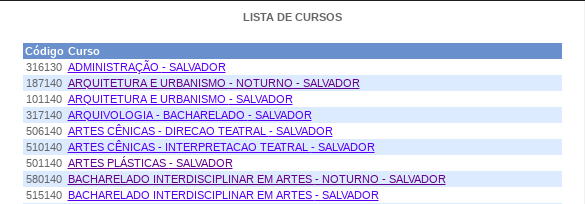
\includegraphics[scale=0.75]{pics/c4/0-cursos.png}
	   \caption{Página com listagem de cursos de graduação da UFBA.}
	   \label{cursos}
\end{figure}
O segundo grupo de endereços encontrado durante a busca manual corresponde a informações refrentes a currículos de curso e espera dois argumentos: ``cdCurso''\footnote{curiosidade: 112140 é o código identificador do curso de ciência da computação na UFBA}, que representa  o código identificador do curso de graduação em questão e ``PerCursoInicial'', que representa o currículo daquele curso. O endereço para o curso de Ciência da Computação da UFBA com o curriculo 2013.2 é:

\url{https://alunoweb.ufba.br/SiacWWW/CurriculoCursoGradePublico.do?cdCurso=112140&nuPerCursoInicial=20132}

A Figura \ref{ementa} exibe a página de detalhes de um currículo, da qual é possível obter as durações mínima e máxima de um currículo, o código do currículo e os diferentes tipos de carga horária. 

\begin{figure}[H]
    \centering
    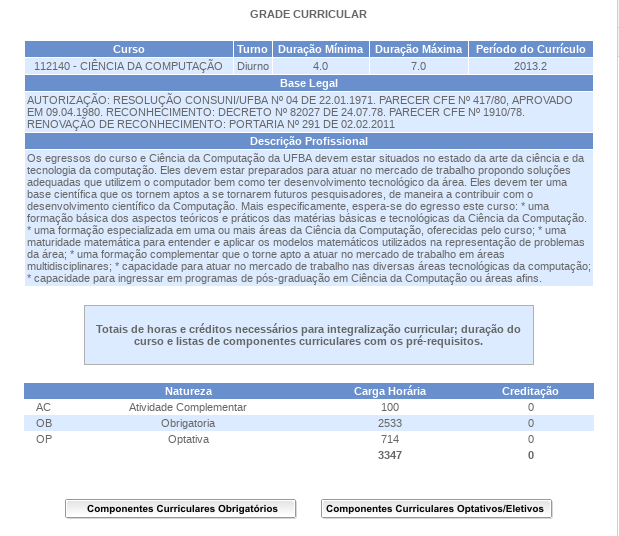
\includegraphics[scale=0.75]{pics/c4/1-ementa.png}
    \caption{Página de detalhes sobre o currículo de um curso.}
    \label{ementa}
\end{figure}

Nessa página de detalhes do currículo (Figura~\ref{ementa}) é possível encontrar dois links que precisam ser acessados através dessa página. Os links correspondem às listagens de disciplinas obrigatórias e disciplinas optativas. A lista de disciplinas obrigatórias agrupa as disciplinas por semestre. Cada disciplina de ambas as listas é representada pelo código única de disciplina, nome da disciplina e é acompanhada por sua natureza e os códigos de seus pré-requisitos, como mostra a Figura~\ref{requireds}.

Após a seleção das páginas fonte, iniciou-se a construção de um sistema de extração de dados da web focado em resolver as necessidades do MeForma2. Esse tipo de sistema é conhecido como Sistema de Web Scraping. O Web Scraping envolve o processo de consultar uma origem, recuperar a página de resultados e analisar a página para obter os resultados \cite{salerno2006method}.

O sistema de web scraping do MeForma2, apelidado de CMF, trabalha em duas etapas que se intercalam durante a recuperação de dados. As etapas correspondem aos sistemas de Web Crawler e Web Wrapper.

\begin{figure}[H]
    \centering
    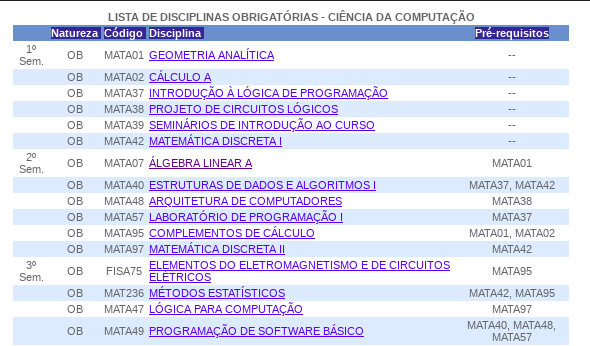
\includegraphics[scale=0.75]{pics/c4/2-requireds.png}
    \caption{Página com listagem de disciplinas obrigatórias.}
    \label{requireds}
\end{figure}

\section{Web Crawler}

Um \textit{Web Crawler}, ou simplesmente \textit{crawler}, é um programa que percorre automaticamente a estrutura de hiperlink da Web e faz o download de cada página vinculada para um armazenamento local \cite{liu}. Quando utilizado para fins de extração de dados, o \textit{crawler} deve identificar e guardar as páginas que contém os dados procurados para futura extração.

A problemática encontrada no desenvolvimento do \textit{crawler} para o MeForma2 foi que as páginas fonte não estavam conectadas. Os links das páginas de currículos não são alcançáveis a partir da página de listagem de cursos e, para acessar uma página de currículos, é necessário saber qual currículo se quer acessar e qual o código do curso referente ao currículo, informações difíceis de se obter manualmente. Contudo, a página de listagem de cursos possui, para cada curso, um endereço para uma lista de disciplinas do curso (sem seus pré-requisitos) que possui um padrão similar ao endereço fonte dos detalhes de um curso:

\url{https://alunoweb.ufba.br/SiacWWW/ListaDisciplinasEmentaPublico.do?cdCurso=316130\&nuPerCursoInicial=20111}.

Visto que o grupo de endereços encontrado na página de lista de cursos contém os parâmetros necessários para carregar a página de detalhes de um currículo, tudo o que o sistema precisou fazer foi, ao alcançar um endereço desse grupo, substituir a expressão ``ListaDisciplinasEmentaPublico'' pela expressão ``CurriculoCursoGradePublico'' antes de navegar no endereço.

\section{Web Wrapper}
O \textit{web wrapper} é um sistema de extração de dados de uma página web. O objetivo de um sistema de \textit{web wrapper}, ou simplesmente \textit{wrapper} é encontrar os dados dentro da estrutura de uma página, extraí-los, estruturá-los (conforme a finalidade para a qual está sendo executado), e exportá-los para uso futuro. De acordo com \cite{liu}, um \textit{wrapper} pode utilizar três diferentes abordagens:
\begin{itemize}
    \item Abordagem manual: Ao observar uma página da \textit{Web} e seu código-fonte, o programador humano localiza alguns padrões e, em seguida, grava um programa para extrair os dados de destino.
    \item \textit{Wrapper induction}: Nessa abordagem, um conjunto de regras de extração é aprendido a partir de uma coleção de páginas ou registros de dados rotulados manualmente.
    \item Extração automatizada: Com uma única ou várias páginas, ele encontra automaticamente padrões ou gramáticas para a extração de dados. Como essa abordagem elimina o esforço de rotulagem manual, ela pode ampliar a extração de dados para um grande número de sites e páginas.
\end{itemize}

Como o escopo do \textit{wrapper} para o MeForma2 é bem definido, pequeno e limitado, a abordagem escolhida foi a abordagem manual. Foi feita uma inspeção na estrutura das páginas HTML que seriam exploradas pelo \textit{wrapper}, identificou-se os padrões de posicionamento dos dados nas páginas, e então desenvolveu-se o \textit{wrapper}.

\section{Funcionamento}

Esta seção descreve o funcionamento do CMF. O algoritmo do CMF funciona como segue:

\begin{enumerate}
    \item O \textit{crawler} lê a URL de entrada (lista de cursos).
    \item O \textit{crawler} faz o download da página referente ao endereço da URL.
    \item O \textit{crawler} é finalizado.
    \item O \textit{wrapper} é iniciado.
    \item Um laço explora a lista de cursos e cria um objeto PHP para cada curso, com as informações disponíveis na página, incluindo a URL para a lista de disciplinas sem pré-requisitos que é substituída pela URL de detalhes do curriculum do curso.
    \begin{minted}{php}
        <?php
        $course = (object)[
            "code" => $td->textContent,
            "name" => Dict::normalize($td->nextSibling->textContent),
            "page" => str_replace("ListaDisciplinasEmentaPublico.do",
                "CurriculoCursoGradePublico.do", 
                "https://alunoweb.ufba.br".
                    $td->nextSibling->firstChild->getAttribute("href")
            )
        ];
        ?>
        \end{minted}
    \item O \textit{wrapper} é finalizado.
    \item Cada objeto é adicionado a um array de cursos.
    \item Um laço percorre o array de objetos de cursos.
    \item O \textit{crawler} é reiniciado utilizando a URL de detalhes do curriculum do próximo curso do array como fonte.
    \item O \textit{crawler} faz o download de cada página de curso e das páginas de disciplinas que são alcançadas durante a navegação.
    \item Assim que o download de uma página de curso e das suas páginas de disciplinas termina, o \textit{crawler} é finalizado.
    \item O \textit{wrapper} é iniciado para as novas páginas recuperadas pelo \textit{crawler}.
    \item O \textit{wrapper} explora os dados do curso, e agrega esses dados ao objeto referente ao curso criado no passo 5.
    \item O \textit{wrapper} explora a página de disciplinas obrigatórias.
    \item Um array de disciplinas obrigatória é criado, onde cada disciplina é um objeto que contém, dentre outros atributos, uma lista com os códigos de suas disciplinas pré-requisito.
    \item O array de disciplinas obrigatórias é agregado ao objeto referente ao curso criado no passo 5.
    \item Um array de disciplinas optativas é criado, analogamente ao passo 15.
    \item O array de disciplinas optativas é agregado ao objeto referente ao curso criado no passo 5.
    \item Os passos 9 - 17 se repetem para cada curso.
    \item O array de cursos que, nesse momento, contém todos os cursos, com todos os detalhes que se desejava explorar, incluindo as disciplinas que compõem o currículo vigente é convertido para o formato JSON.
    \item O JSON de cursos é salvo em arquivo.
\end{enumerate}

A execução padrão do CMF explora todos os cursos de graduação da UFBA exibidos na página de listagem de cursos, e os armazena em um arquivo JSON. Contudo, em algumas situações, é desejável executar o CMF para uma lista específica de cursos. Nesse caso, o sistema recebe um array com os códigos de identificação dos cursos desejados e, antes da execução do passo 4, a lista de cursos é filtrada para que somente os cursos desejados sejam recuperados.

Após a execução do CMF, um outro algoritmo, o MTransfer, se encarrega de ler o conteúdo exportado pelo CMF e inserir no banco de dados do sistema.
\chapter{Avaliação e Resultados}
Neste capítulo serão mostradas uma avaliação heurística, uma avaliação de relevância da aplicação, uma pesquisa de satisfação dos usuários, sugestões enviadas por usuários e estatísticas de uso da aplicação. Todos esses recursos foram utilizados para estimar a qualidade do software MeForma2.

Determinar a qualidade de um software é uma atividade complexa e imprecisa. Em seu trabalho sobre Visões de Qualidade, \cite{garvin} analisa a qualidade sob a perspectiva de diversas áreas do conhecimento, como filosofia, economia e marketing. Ele afirma que ``a qualidade é um conceito complexo que possui muitas faces''. \cite{garvin} considera que a qualidade pode ser descrita sob cinco perspectivas: 
\begin{itemize}
    \item A visão transcendental - que vê qualidade como algo que pode ser reconhecido, mas não definido.
    \item A visão do usuário - que vê qualidade como adequação para um propósito.
    \item A visão do fabricante - que considera a qualidade como conformidade com a especificação.
    \item A visão do produto - vê a qualidade como ligada às características inerentes do produto.
    \item A visão baseada em valor - considera a qualidade como dependente do valor que um cliente está disposto a pagar por ela.
\end{itemize}

Neste trabalho optou-se por avaliar a qualidade do software principalmente sob a perspectiva do usuário. Associou-se a qualidade do software em questão à reação dos usuários ao mesmo. Entendeu-se que se os usuários classificam o software como adequado para o fim proposto, consideram-se satisfeitos com os recursos que o software oferece e estão dispostos a indicá-lo a outras pessoas, então esse é um software de qualidade.

\section{Avaliação Heurística}

A Avaliação Heurística é um método de avaliação de usabilidade de software proposto por \cite{nielsen}. O método permite ao avaliador examinar uma solução para tentar antever as possíveis consequências de certas decisões de design. Esse método de avaliação é categorizado como método de avaliação por inspeção e não envolve os usuários.

Para realizar a avaliação, utilizou-se um conjunto de diretrizes de usabilidade, definidas por Nielsen, chamadas de heurísticas de usabilidade. Uma heurística é uma regra que funciona na prática, mas não exige uma explicação teórica. Foram enumeradas 10 heurísticas:

\begin{itemize}
    \item H1: Visibilidade do status do sistema - O sistema deve sempre manter os usuários informados sobre o que está acontecendo através de \textit{feedback}\footnote{resposta rápida e apropriada} rápido e apropriado.
    \item H2: Correspondência entre o sistema e o mundo real - O sistema deve falar a linguagem do usuário, 0,com palavras, frases e conceitos familiares ao usuário. Ele deve seguir convenções do mundo real, fazendo informações aparecem em uma ordem lógica e natural. 
    \item H3: Controle e liberdade para o usuário - Muitas vezes os usuários podem realizar ações por engano. A aplicação deve permitir que os usuários desfaçam e refaçam suas ações.
    \item H4: Consistência e padronização - O sistema deve seguir as convenções existentes, utilizando sempre as mesmas palavras e ícones para as mesmas ações.
    \item H5: Prevenção de Erros - Um sistema que evite que erros ocorram é ainda melhor que um sistema com boas mensagens de erro.
    \item H6: Reconhecimento ao invés de memorização - O usuário não deve ter que lembrar de informações de outras partes do sistema. Instruções de uso do sistema devem estar sempre visíveis ou serem facilmente encontradas.
    \item H7: Flexibilidade e eficiência no uso - A utilização do sistema deve ser agilizada pelo uso de atalhos.
    \item H8: Design estético e minimalista - O sistema não deve exibir informações desnecessárias, pois elas irão competir com as necessárias.
    \item H9: Ajuda para reconhecer, diagnosticar e se recuperar de erros - Mensagens de erro devem ser claras, indicar o problema e sugerir uma solução.
    \item H10: Ajuda e documentação - O ideal é que o sistema não precise de documentação para ser usado. Pode-se incluir diálogos de ajuda e/ou de uma documentação sucinta.
\end{itemize}

As infrações encontradas foram julgadas a partir da classificação de severidade explicada na Tabela~\ref{severidade}. Esse modelo de classificação foi proposto por \cite{nielsen}.

\begin{table}[H]
\caption{Classificação de severidade de problemas de usabilidade.}
\label{severidade}
\begin{tabular}{ |c|c| } 
 \hline
 Severidade & Explicação \\
 \hline
 0 & Não é encarado como um problema de usabilidade. \\
 \hline
 1 & Problema estético - a ser corrigido apenas se houver tempo disponível. \\
 \hline
 2 &  Problema pequeno - baixa prioridade para sua correção. \\
 \hline
 3 & Problema grande - alta prioridade para sua correção. \\
 \hline
 4 &  Problema catastrófico - é extremamente necessário corrigir. \\
 \hline
\end{tabular}
\end{table}

Para guiar a avaliação, foram selecionados oito cenários de uso do sistema que contemplam as principais telas:

\begin{enumerate}
    \item Como usuário, gostaria de me cadastrar no sistema;
    \item Como usuário, gostaria de selecionar as disciplinas que já cursei;
    \item Como usuário, gostaria de visualizar os pré-requisitos de uma disciplina;
    \item Como usuário, gostaria de cadastrar uma carga horária;
    \item Como usuário, gostaria de cadastrar um semestre;
    \item Como usuário, gostaria de contabilizar minhas faltas em uma disciplina;
    \item Como usuário, gostaria de importar dados do SIAC;
    \item Como usuário, gostaria de visualizar minha completude de curso.
\end{enumerate}

A Tabela~\ref{avaliacaoheuristica} lista e classifica as infrações encontradas no MeForma2 pelo método de avaliação heurística. Nenhuma infração foi classificada com Severidade 4, ou seja, não houveram problemas catastróficos durante a análise, além disso, os demais problemas não exigem mudanças nas regras de negócio da aplicação, pois tratam-se apenas de correções visuais e adição de textos. 

O resultado da avaliação indica que o sistema possui uma interface bem resolvida e intuitiva. O que significa dizer que os usuários terão pouca ou nenhuma dificuldade em utilizar a interface.

\begin{table}[H]
\begin{center}
\caption{Infrações encontradas no MeForma2 pela avaliação heurística.}
\begin{tabular}{ |p{3cm}|c|c|c|p{5.5cm}| }
\hline
 \textbf{Problema} & \textbf{Cenário} & \textbf{Heurísticas} & \textbf{Severidade} & \textbf{Explicação} \\ 
 \hline
 Confirmação de e-mail e senha & 1 & H5 & 3 & O cadastro não exige confirmação de e-mail ou senha, caso o usuário insira dados inválidos, ele pode não conseguir utilizar o sistema posteriormente \\
 \hline
 Estilo dos campos do formulário & 1 & H7 & 1 & Os campos do formulário são diferentes dos utilizados pelo \textit{Android}, o que pode causar confusão ao usuários da versão mobile. \\
 \hline
 Múltiplas ações ao clicar em disciplina & 2 & H5 & 3 & Existem duas ações ao clicar nos cartões das disciplinas. Elas se diferenciam pelo tempo de clique. Isso pode causar confusão e impedir a descoberta de funcionalidades. \\
 \hline
 Legenda na identificação de pré-requisitos & 3 & H6 & 1 & Não existe legenda para indicar qual a cor que representa um pré-requisito e qual a cor que representa uma dependência, mas foi considerado um problema pequeno, pois o usuário pode visualizar a organização temporal das disciplinas. \\
 \hline
 Mensagem de confirmação de alteração de Carga Horária & 4 & H1 & 2 & Não existem mensagens de sucesso após ações de criar, editar ou excluir uma carga horária, contudo, o usuário pode identificar a mudança na lista imediatamente. \\
 \hline
 Falta de informação ao importar dados do SIAC & 7 & H10 & 2 & O sistema não deixa claro quais dados serão importados do SIAC, podendo deixar o usuário confuso sobre o correto funcionamento da funcionalidade. \\
 \hline
\end{tabular}
\end{center}
\label{avaliacaoheuristica}

\end{table}

\section{Avaliação de Relevância da Aplicação}

A Avaliação de Relevância é uma pesquisa realizada com os usuários do MeForma2, grupo composto por estudantes de graduação da Universidade Federal da Bahia, onde a opinião dos usuários determina a relevância da aplicação. A pesquisa foi realizada de modo anônimo.

A avaliação levou em consideração 3 fatores para determinar a relevância do MeForma2 que combinam com o objetivo da aplicação:
\begin{itemize}
    \item É uma ferramenta que ajuda o estudante a organizar sua vida acadêmica;
    \item É uma ferramenta que ajuda o estudante a entender o que é preciso para alcançar a formatura;
    \item É uma ferramenta que ajuda o estudante a ser responsável com o curso;
\end{itemize}

A pesquisa obteve 62 respostas em 13 dias e o resultado apontou o MeForma2 como uma ferramenta relevante para os cursos de graduação da UFBA. Cada critério foi avaliado com notas de 1 a 5, onde 1 significa que o MeForma2 é totalmente irrelevante para aquele quesito e 5 representa que o MeForma2 é muito relevante para aquele quesito.

As Figuras~\ref{organize}, \ref{graduate} e \ref{responsability} exibem os resultados da pesquisa de relevância da aplicação. Os resultados indicam que o MeForma2 está ajudando os estudantes que participaram da avaliação a se organizarem e a compreenderem melhor sua vida acadêmica, além de alertá-los sobre a responsabilidade que eles tem que ter com o próprio curso.

\begin{figure}[H]
	   \centering
	   		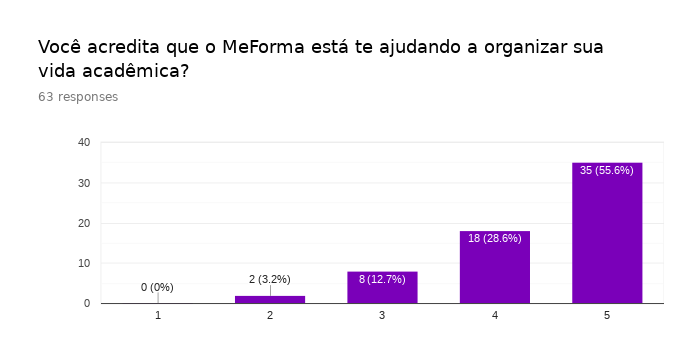
\includegraphics[scale=0.65]{pics/c5/0-organize.png}
	   \caption{Avaliação sobre ajuda com organização de vida acadêmica}
	   \label{organize}
\end{figure}
\begin{figure}[H]
	   \centering
	   		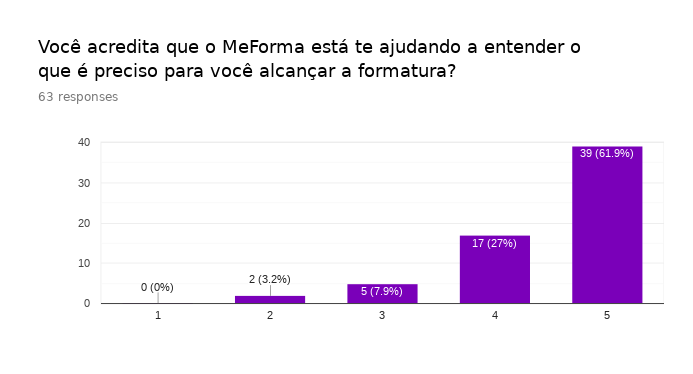
\includegraphics[scale=0.65]{pics/c5/1-graduate.png}
	   \caption{Avaliação sobre entendimento de pré-requisitos para formatura.}
	   \label{graduate}
\end{figure}
\begin{figure}[H]
	   \centering
	   		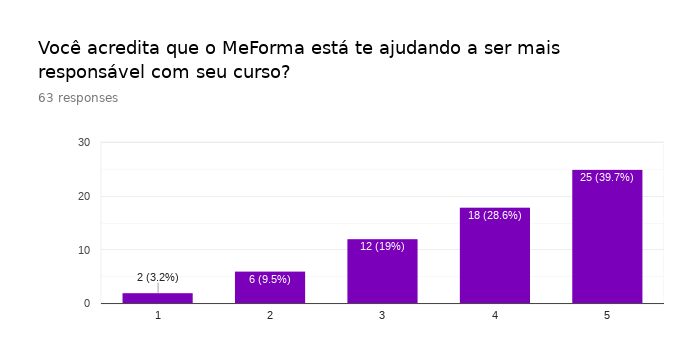
\includegraphics[scale=0.65]{pics/c5/2-responsability.png}
	   \caption{Avaliação sobre responsabilidade com o curso.}
	   \label{responsability}
\end{figure}

\section{Pesquisa de Satisfação}

Esta pesquisa teve a intenção de avaliar dois fatores considerados como fundamentais para o crescimento do MeForma2: o quanto os usuários estavam satisfeitos com o sistema e o quanto eles estavam dispostos a indicar o sistema a outras pessoas. Esses quesitos foram apresentados aos entrevistados como duas perguntas, as quais poderiam ser respondidas com notas de 1 a 5:
\begin{itemize}
    \item Qual o seu nível de satisfação com o MeForma?
    \item Você indicaria o MeForma a um amigo ou colega?
\end{itemize}

A decisão de realizar uma pesquisa de satisfação e os quesitos de avaliação escolhidos tiveram como inspiração as pesquisas de satisfação de cliente realizadas na área de marketing. Segundo Lobos \cite{lobos} "a melhor propaganda é um cliente satisfeito" e "clientes satisfeitos tornam-se apóstolos". Entendeu-se que usuários satisfeitos permanecem utilizando a aplicação e que usuários dispostos a indicar a aplicação atraem novos usuários. 

Os usuários que responderam a pesquisa foram classificados em 3 categorias de acordo com a pergunta "Você indicaria o MeForma a um amigo ou colega?":

\begin{itemize}
    \item Detratores - Usuários que deram nota menor que 3. São pessoas insatisfeitas que podem impedir o crescimento da aplicação através do boca-a-boca negativo.
    \item Neutros - Usuários que deram nota 3 e 4. São clientes satisfeitos, mas que possuem queixas importantes sobre a aplicação. São considerados como vulneráveis a ofertas da concorrência.
    \item Promotores - Usuários que deram nota 5. São clientes leais que vão continuar utilizando a aplicação e a indicarão para outras pessoas.
\end{itemize}

Considerou-se que usuários que demonstraram existir a possibilidade de não indicar o MeForma2 para outras pessoas possuem alguma queixa sobre a aplicação.

\begin{figure}[H]
	   \centering
	   		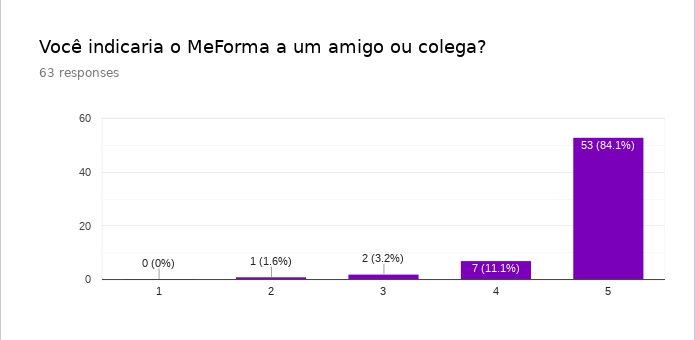
\includegraphics[scale=0.65]{pics/c5/3-share.png}
	   \caption{Disposição dos usuários em indicar o MeForma a outras pessoas.}
	   \label{nps}
\end{figure}

O Figura \ref{nps} mostra a reação dos usuários à pergunta sobre indicar o sistema a outra pessoa. Os resultados indicam que 84,1\% dos entrevistados são Promotores, 1,6\% são Detratores e 14,3\% (3,2\% + 11,1\%) são Neutros. Esse resultado indica que o MeForma2 tem grandes chances de se tornar popular através de divulgação informal proveniente dos próprios usuários, mesmo que alguns deles tenham reclamações a fazer.

\section{Estatísticas de uso da aplicação}

Um diferencial importante trazido pelo MeForma2 foi a publicação de uma plataforma WEB. Muitos usuários da primeira versão do MeForma solicitaram uma versão WEB e, pela característica da aplicação, de ser um serviço de consulta de dados, os usuários se mostravam resistentes a instalar o aplicativo em seus dispositivos.

A divulgação da versão WEB fez com que, não só o número de usuários aumentasse rapidamente, mas também fez com que os acessos ao sistema aumentassem.

Os dados que serão apresentados nesta seção foram computados entre os dias 28 de Outubro de 2018 (Data de lançamento do MeForma2) e 16 de Novembro de 2018, um total de 20 dias.

A Figura \ref{installs} mostra o número de instalações do aplicativo para Android em função do tempo. A linha vertical marca o dia de lançamento do MeForma2. A imagem mostra um crescimento no número de usuários do aplicativo, que saltou de 104 para 141 usuários. A linha tracejada corresponde ao mês anterior, possibilitando visualizar uma queda no número de usuários entre setembro e outubro, e o crescimento entre outubro e novembro.   

\begin{figure}[H]
	   \centering
	   		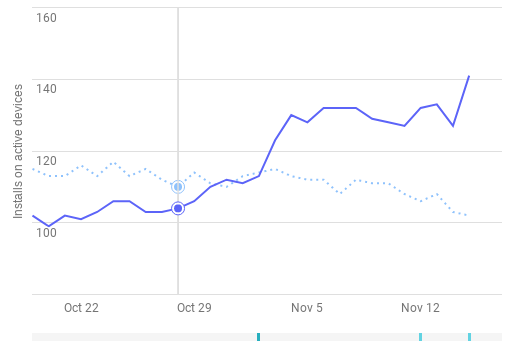
\includegraphics[scale=0.85]{pics/c5/5-installs.png}
	   \caption{Instalações do MeForma para Android.}
	   \label{installs}
\end{figure}

A Figura \ref{web} mostra o número de usuários ativos da versão WEB do MeForma2 em função do tempo. A imagem mostra que a versão WEB teve um número muito maior de usuários, 479 contra 141 do aplicativo. Isso demonstra a preferência do público do MeForma2 pela versão WEB, informação reforçada pelo fato de que na versão web existe o link de download do aplicativo, e as pessoas dão preferência por permanecer na versão web.

\begin{figure}[H]
	   \centering
	   		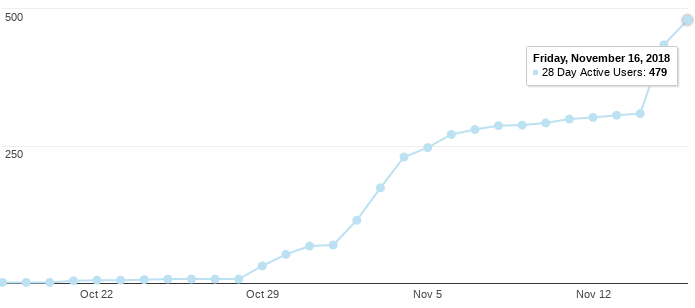
\includegraphics[scale=0.65]{pics/c5/6-active.png}
	   \caption{Utilização do MeForma para WEB}
	   \label{web}
\end{figure}

A Figura \ref{sessions} mostra os dispositivos pelos quais os usuários acessaram a versão WEB do MeForma2.

\begin{figure}[H]
	   \centering
	   		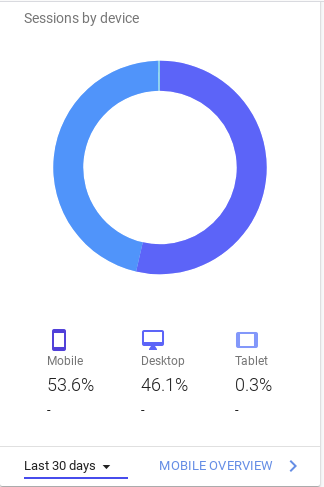
\includegraphics[scale=0.65]{pics/c5/4-sessions.png}
	   \caption{Distribuição do MeForma2 WEB entre os dispositivos.}
	   \label{sessions}
\end{figure}

Uma outra contribuição interessante da versão WEB foi a inclusão de usuários de plataformas mobile diferentes do Android, uma vez que o aplicativo mobile só está disponível para Android. A Figura \ref{mobiles} mostra que o MeForma WEB foi utilizados por usuários do IOS e do Windows, sendo que os usuários do IOS correspondem a 25\% dos usuários da versão WEB em dispositivos móveis.

\begin{figure}[H]
	   \centering
	   		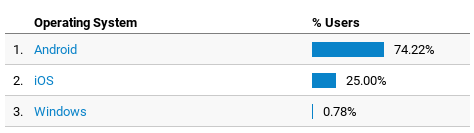
\includegraphics[scale=0.75]{pics/c5/7-mobiles.png}
	   \caption{Distribuição dos usuários mobile por dispositivo.}
	   \label{mobiles}
\end{figure}

A Figura \ref{topcourses} mostra a lista dos 10 cursos que mais utilizam o MeForma. Dando destaque para a porcentagem de usuários dos cursos de Ciência da Computação e Sistemas de Informação que são os cursos que mais se interceptam com o ciclo social do desenvolvedor, e que por causa disso recebem mais informações sobre a aplicação. Levando à intuição de que para se tornar popular entre todos os estudantes da UFBA, a aplicação precisa de um trabalho de divulgação ativo. Até então, toda a divulgação foi feita por Facebook e E-mail.

\begin{figure}[H]
	   \centering
	   		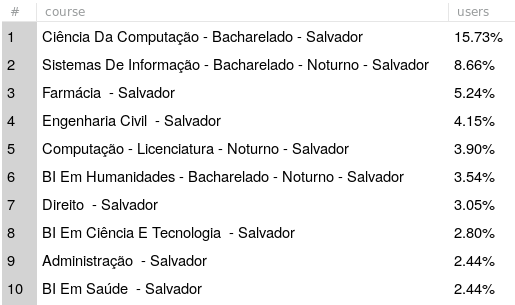
\includegraphics[scale=0.75]{pics/c5/8-topcourses.png}
	   \caption{10 cursos que mais utilizam o MeForma.}
	   \label{topcourses}
\end{figure}

Os dados apresentados até aqui são bastante úteis para entender o público do MeForma2.

\section{Sugestões dos Usuários}

As pesquisas realizadas com os usuários continham um campo para envio de comentários. No total foram enviados 23 comentários, dos quais 14 continham mensagens positivas de parabenização ou elogio.

\say{O aplicativo está muito bom, está atendendo minhas necessidades de forma excelente. Parabéns}

\say{Ótima aplicação, não consigo me imaginar sem ela. Totalmente excepcional!}

\say{Me ajudou bastante pra saber quanto eu faltava de carga horária.}

\say{O que eu mais esperava era a versão web. Amém!}

Dentre os 23 comentários, 7 continham alguma sugestão de melhoria para a aplicação.
 
\say{Acho que na parte de faltas em cada matéria, poderia ter uma opção de ordenar pela matéria com maior número de faltas.}
 
\say{Como venho de transferência interna, no início, tomei um pequeno susto ao perceber que o MeForma não importou automaticamente os dados de disciplinas que eu fiz aproveitamento de estudos (classificados no SIAC como "Dispensado"), seria bacana se isso já fosse feito direto na importação de dados de alguma forma.}
 
\say{Talvez mudar a cor do botão "importar do SIAC" para ficar mais visível}
 
 \say{Ao clicar para recuperar senha, sugiro mais instruções no e-mail.}
 
2 dos usuários demonstraram confusão em seus comentários.
 
\say{Não entendi porque em currículo só existem 3 opções e só vai até 2013.2}
 
\say{Não entendi o menu "CH", para mim só aparece que não tenho nada, mesmo eu tendo a carga horária optativa.}

Não houveram comentários negativos, o que indica que a plataforma, mesmo não agradando totalmente 100\% dos usuários, não desagrada ninguém ao ponto de a pessoa fazer uma reclamação direta.

\section{Interesse Externo}

Estudantes de outras instituições ao ter algum contato com o MeForma enviaram mensagens demonstrando interesse e questionando se era possível utilizar em sua instituição. A Tabela \ref{interesse} mostra as instituições representadas e a quantidade de contatos estabelecidos.

\begin{table}[H]
\begin{center}
\begin{tabular}{ |p{10cm}|p{2cm}| }
\hline
Instituição & Contatos \\
\hline
UFpel - Universidade Federal de Pelotas  & 3 \\
\hline
UFRB - Universidade Federal do Recôncavo da Bahia & 3 \\
\hline
Estácio - Universidade Estácio de Sá & 2 \\
\hline
UFSJ - Universidade Federal de São João Del Rei & 2 \\
\hline
Anhanguera & 1 \\
\hline
Colégio Estadual Professor José Accioli & 1 \\
\hline
Estacio FIC do Ceará & 1 \\
\hline
Faculdade JK - Santa maria & 1 \\
\hline
Faculdade Nobre & 1 \\
\hline
FTC - Faculdade de Tecnologia e Ciências& 1 \\
\hline
IFBA - Instituto Federal da Bahia & 1 \\
\hline
IFSC - Instituto Federal de Santa Catarina & 1 \\
\hline
UCS - Universidade de Caxias do Sul & 1 \\
\hline
UFES - Universidade Federal do Espírito Santo & 1 \\
\hline
UFPB - Universidade Federal da Paraíba & 1 \\
\hline
UFPE - Universidade Federal de Pernambuco & 1 \\
\hline
UFS - Universidade Federal de Sergipe& 1 \\
\hline
UNIFACS - Universidade Salvador & 1 \\
\hline
UNIMEP - Universidade Metodista de Piracicaba  & 1 \\
\hline
Universidade Castelo Branco & 1 \\
\hline
UESB - Universidade Estadual do Sudoeste da Bahia  & 1 \\
\hline
UFRR - Universidade Federal de Roraima & 1 \\
\hline
UFOB - Universidade Federal do Oeste da Bahia  & 1 \\
\hline
URGS - Universidade do Rio Grande do Sul& 1 \\
\hline
\end{tabular}
\end{center}
\label{interesse}
\caption{Instituições de ensino representadas na demonstração de interesse pelo MeForma}
\end{table}

\section{Otimização do aplicativo para Android}

Um dos parâmetros para determinar a qualidade de um aplicativo para Android é o tempo de início do aplicativo. De acordo com a documentação do Android, os usuários esperam que os aplicativos sejam responsivos e rápidos para carregar. Um aplicativo com um tempo de início lento não atende a essa expectativa e pode ser decepcionante para os usuários. Esse tipo de experiência insatisfatória pode fazer com que um usuário avalie mal um aplicativo na Play Store ou até mesmo abandone o aplicativo completamente.

O MeForma teve duas grandes versões do aplicativo lançadas, e sete versões de correção e melhoria de funcionalidades. A Figura~\ref{startuptime} mostra o gráfico que compara o desempenho com relação ao tempo de início das versões do aplicativo MeForma. Os valores utilizados para construir o gráfico da Figura~\ref{startuptime} foram obtidos através de uma média aritmética entre 5 cronometragens de inicialização feitas para cada versão. A Tabela~\ref{startuptime2} mostra os tempos em segundos obtidos em cada teste e a média obtida.

\begin{figure}[H]
	   \centering
	   		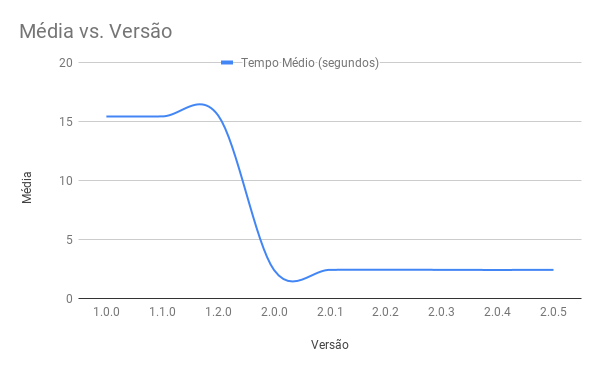
\includegraphics[scale=0.65]{pics/c5/9-startuptime.png}
	   \caption{Tempo médio de inicialização do MeForma por versão e subversão.}
	   \label{startuptime}
\end{figure}

\begin{table}[H]
\begin{center}
\caption{Tempo de inicialização do MeForma por versão.}
\begin{tabular}{ |c|c|c|c|c|c|c| }
\hline
 \textbf{Versão} & \textbf{Teste 1} & \textbf{Teste 2} & \textbf{Teste 3} & \textbf{Teste 4} & \textbf{Teste 5} & \textbf{Média (s)} \\ 
 \hline
 \textbf{1.0.0} & {15.78} &	{15.41} &	{15.29} &	{15.42} &	{15.8} &	{15.42} \\
 \hline 
 \textbf{1.1.0} & {15.43} &	{15.35} &	{15.55} &	{15.29} &	{15.43} &	{15.43} \\
 \hline 
 \textbf{1.2.0} & {15.38} &	{15.55} &	{15.51} &	{15.48} &	{15.7} &	{15.51} \\
 \hline 
 \textbf{2.0.0} & {2.3} &	{2.43} &	{2.41} &	{2.43} &	{2.36} &	{2.41} \\
 \hline 
 \textbf{2.0.1} & {2.54} &	{2.3} &	{2.4} &	{2.43} &	{2.44} &	{2.43} \\
 \hline 
 \textbf{2.0.2} & {2.49} &	{2.22} &	{2.44} &	{2.2} &	{2.5} &	{2.44} \\
 \hline 
 \textbf{2.0.3} & {2.38} &	{2.5} &	{2.45} &	{2.43} &	{2.38} &	{2.43} \\
 \hline 
 \textbf{2.0.4} & {2.44} &	{2.42} &	{2.46} &	{2.41} &	{2.35} &	{2.42} \\
 \hline 
 \textbf{2.0.5} & {2.48} &	{2.43} &	{2.45} &	{2.34} &	{2.25} &	{2.43} \\
 \hline 
\end{tabular}
\end{center}
\label{startuptime2}

\end{table}

É possível perceber, através dos dados apresentados, que houve uma queda de aproximadamente 13 segundos no tempo de inicialização do aplicativo. Isso se justifica pela mudança de estratégia que houve no carregamento das páginas do aplicativo. A primeira versão do MeForma utilizava uma estratégia chamada de \textit{Eager Loading} e o MeForma2 utiliza uma estratégia chamada de \textit{Lazy Loading}:
\begin{itemize}
    \item \textit{Eager Loading} - Todas as páginas do aplicativo são carregadas antes da inicialização. Isso significa que o \textit{WebView} precisa carregar, analisar e interpretar o javascript de cada página para tornar o aplicativo utilizável.
    \item \textit{Lazy Loading} - Apenas o mínimo necessário para a inicialização do aplicativo é carregado. Em termos práticos, significa que apenas o javascript necessário para a primeira página deverá ser buscado, analisado e interpretado. A partir daí, toda vez que um recurso específico (como uma página, por exemplo) é necessário, é feito o carregamento por demanda daquele recurso.
\end{itemize}

O principal objetivo da aplicação da técnica de \textit{Lazy Loading} era a redução no tempo de início do aplicativo. A cronometragem de tempo de início exibida na Tabela~\ref{startuptime2} demonstra que o objetivo foi alcançado.

Segundo a documentação do Ionic Framework, a aplicação da técnica de \textit{Lazy Loading} melhora o tempo de inicialização dos aplicativos e reduz o tamanho do pacote. A Tabela~\ref{appsize} mostra os tamanhos dos pacotes referentes às diferentes versões do MeForma. De acordo com a tabela, houve uma redução de aproximadamente 53\% no tamanho do pacote ao compararmos a versão 1.2.0 (última versão referente ao primeiro aplicativo do MeForma) e a versão 2.0.5 (última versão referente ao MeForma2).


\begin{table}[H]
\begin{center}
\caption{Tamanho em MB das versões do MeForma.}
\begin{tabular}{ |c|c| }
\hline
 \textbf{Versão} & \textbf{Tamanho do pacote} \\ 
 \hline
 \textbf{1.0.0} & {4.55 MB} \\
 \hline 
 \textbf{1.1.0} & {5.11 MB} \\
 \hline 
 \textbf{1.2.0} & {5.11 MB} \\
 \hline 
 \textbf{2.0.0} & {2.40 MB} \\
 \hline 
 \textbf{2.0.1} & {2.40 MB} \\
 \hline 
 \textbf{2.0.2} & {2.39 MB} \\
 \hline 
 \textbf{2.0.3} & {2.40 MB} \\
 \hline 
 \textbf{2.0.4} & {2.42 MB} \\
 \hline 
 \textbf{2.0.5} & {2.42 MB} \\
 \hline 
\end{tabular}
\end{center}
\label{appsize}

\end{table}

O principal detalhe na comparação entre as versões do aplicativo é que mesmo possuindo mais funcionalidades do que a versão anterior, o MeForma2 se mostrou mais rápido e mais leve no sentido de ocupar menos espaço no dispositivo do usuário. A escolha da estratégia de carregamento do aplicativo foi fundamental para a obtenção desses resultados.


 
 
\chapter{Conclusão}

Este trabalho apresentou a aplicação MeForma2, seu funcionamento e sua importância para o acompanhamento do progresso dos estudantes de graduação da UFBA em seus respectivos currículos de curso, não só para os próprios estudantes, mas também para os gestores de cada curso.

O processo de desenvolvimento englobou a definição de requisitos, a escolha das linguagens de programação e das ferramentas utilizadas, a escolha das plataformas que receberiam suporte, a modelagem de um banco de dados, a implementação de crawlers, wrappers e da própria aplicação. O resultado final desse processo foi uma aplicação de uso simples e fácil, com uma execução dividida em etapas bastante definidas.

A aplicação foi avaliada por um grupo de usuários através de uma pesquisa de relevância, e estes a consideraram relevante não só para a organização de suas vidas acadêmicas, mas também para entender os pré-requisitos necessários para alcançar a formatura, além de contribuir para torná-los mais responsáveis com seu progresso no curso.

Uma avaliação heurística, mostrou que a aplicação não possui nenhum problema catastrófico de usabilidade e que está adequada para a utilização dos estudantes. Conclusão que foi reforçada pela pesquisa de satisfação realizada com um grupo de usuários que se mostraram contentes com o MeForma2, mesmo que para alguns a aplicação possua pontos que precisem de melhora.

As estatísticas de uso coletadas mostraram um aumento na quantidade de usuários da aplicação e a preferência dos usuários pela versão Web do MeForma2, mostrando que o desenvolvimento da versão web foi uma contribuição importante para os estudantes. Além disso, as estatísticas mostram que a versão web foi importante para o crescimento do MeForma2, pois conseguiu atingir grupos de usuários que o MeForma original não era capaz de atingir, como por exemplo, os usuários de dispositivos Apple.

Dentre as contribuições deste trabalho, se destacam:
\begin{itemize}
    \item O MeForma2 - que já está sendo utilizado pelos estudantes de graduação da UFBA sem restrições.
    \item O MFPAC - que está em versão alpha, sendo utilizado apenas pelo colegiado de Ciência da Computação da Universidade Federal da Bahia.
    \item A pesquisa de fontes de dados sobre disciplinas e cursos na UFBA - que podem ser utilizadas tanto para a melhoria do MeForma2, quanto para a criação de novas aplicações com objetivos diferentes.
    \item O CMF - O capítulo 4 mostrou os passos para construção do \textit{web scraping} CMF e como o mesmo trabalha para obter os dados de disciplinas e cursos da UFBA, o que pode guiar a criação de novos sistemas com fins similares.
\end{itemize}

Sobre o MFPAC e a leitura dos dados obtidos da utilização do MeForma2 pelos estudantes, é importante ressaltar que são ferramentas para auxiliar decisões administrativas, e que não traduzem a realidade com precisão, pois são apenas números. Números esses que podem levar a diferentes conclusões se forem analisados isoladamente, a depender do que está sendo avaliado. Uma decisão administrativa sobre uma disciplina, por exemplo, deve levar em consideração não apenas os números levantados, mas também a opinião dos envolvidos sobre a disciplina, a opinião dos estudantes sobre os professores que ensinam aquela disciplina, a qualidade do ambiente onde a disciplina é lecionada, o conteúdo da ementa, os tipos de avaliação que tem sido aplicados, e uma série de variáveis que influenciam no desempenho dos estudantes. 

Foram identificadas algumas possibilidades de trabalhos e funcionalidades que podem ser desenvolvidos futuramente para agregar mais valor tanto ao MeForma2 quanto aos seus usuários:

\begin{itemize}
    \item Permitir que o usuário realize a pré-matrícula semestral através do sistema - Facilitaria o trabalho dos gestores com relação ao planejamento das disciplinas que serão ofertadas em um determinado semestre.
    \item Sugestão de conjunto de disciplinas para o semestre seguinte - A intenção é sugerir ao estudante um semestre equilibrado no sentido de não se matricular em muitas disciplinas com alto índice de reprovação no mesmo semestre.
    \item Notificação sobre o lançamento da nota das disciplinas que o usuário está cursando no SIAC - Agregaria valor à experiência do usuário.
    \item Agenda de aulas e atividades curriculares - A intenção é ajudar o estudante a se manter alerta sobre sua rotina e compromissos acadêmicos.
    \item Permitir simulação de cumprimento de disciplinas - Útil para auxiliar no planejamento dos semestres.
    \item Sugestão de formas de cumprir carga horária - Permitiria que estudantes que precisam cumprir carga horária descobrissem opções já utilizadas por outros.
    \item Corrigir os problemas apontados pela avaliação heurística.
\end{itemize}

O MeForma2 se mostrou adequado e relevante para os estudantes de graduação da UFBA e divulgá-lo é fundamental para que ele possa atingir seu objetivo com altos índices de qualidade, uma vez que, quanto mais usuários utilizarem o sistema, mais fiéis se tornam os dados que ele exibe. Além disso, o interesse de estudantes de outras instituições de ensino pela aplicação demonstram que a problemática que motivou seu desenvolvimento também está presente na vida acadêmica desses estudantes, e que o MeForma2 tem boas chances de ultrapassar as fronteiras da UFBA.

\phantompart
\postextual
\bibliography{references.bib}
\phantompart
\printindex
\end{document}
